\chapter{Déploiement de l'infrastructure IT}

%\markboth{Chapitre 2 }{Déploiement de l'infrastructure IT} %pour afficher l'entete
%\addcontentsline{toc}{chapter}{Chapitre 2 : Déploiement de l'infrastructure IT}


\section{Introduction}

Le déploiement de l'infrastructure informatique est une étape cruciale pour  Zeta Engineering. Après avoir choisi la méthodologie en cascade, nous sommes prêts à passer à la mise en place de l'infrastructure nécessaire à la réalisation du projet.

Dans ce chapitre, nous détaillons les différentes étapes du déploiement de l'infrastructure IT, notamment la mise en place du réseau, la sélection des équipements matériels et logiciels.

Nous expliquons également les choix techniques que nous avons effectués pour répondre aux exigences de l'entreprise et assurer une infrastructure robuste et sécurisée. Tout au long de ce chapitre, nous détaillons les différentes étapes du déploiement et expliquons les raisons de nos choix techniques afin de permettre une compréhension approfondie de notre approche.

\section{Outils et technologies utilisés}

Dans cette partie, nous allons détailler les différents outils et technologies que nous avons utilisés pour établir l'infrastructure réseau IT et SI nécessaire à la mise en place.

Nous abordons tout d'abord le matériel que nous avons sélectionné et configuré pour répondre aux besoins de l'entreprise, dans la section 2.2.1.

Ensuite, nous présentons l'environnement IT que nous avons mis en place, en décrivant les différentes technologies et logiciels utilisés pour assurer une infrastructure stable, performante et sécurisée, dans la section 2.2.2.

Cette présentation détaillée nous permettra de mieux comprendre les choix que nous avons effectués pour répondre aux exigences de l'entreprise et assurer une mise en œuvre réussie de notre projet.

\subsection{Matériels utilisés}

Dans cette sous-section, nous présentons le matériel utilisé, notamment les commutateurs, le pare-feu et les serveurs, sous forme d'un tableau \ref{1}.


\begin{table}[H]
\begin{center}
\begin{tabular}{|c{3cm}|c{3cm}|l{10cm}|}
\hline
\textbf{Image de l'équipement}         & \textbf{Nom de l'équipement}   & \textbf{Fonctionnalité} \\
\hline
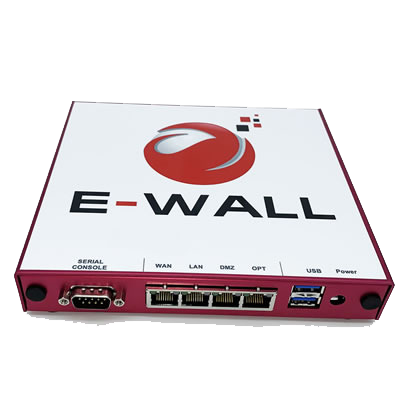
\includegraphics[width=3cm]{Images/ewall.png} & E-Wall Pare-Feu & E-Wall est une solution de sécurité essentielle pour protéger les réseaux informatiques contre les menaces externes. 

Son utilisation permet de renforcer la sécurité, de contrôler le trafic réseau et de détecter les activités malveillantes, contribuant ainsi à la préservation de l'intégrité, de la confidentialité et de la disponibilité des données. \\
\hline
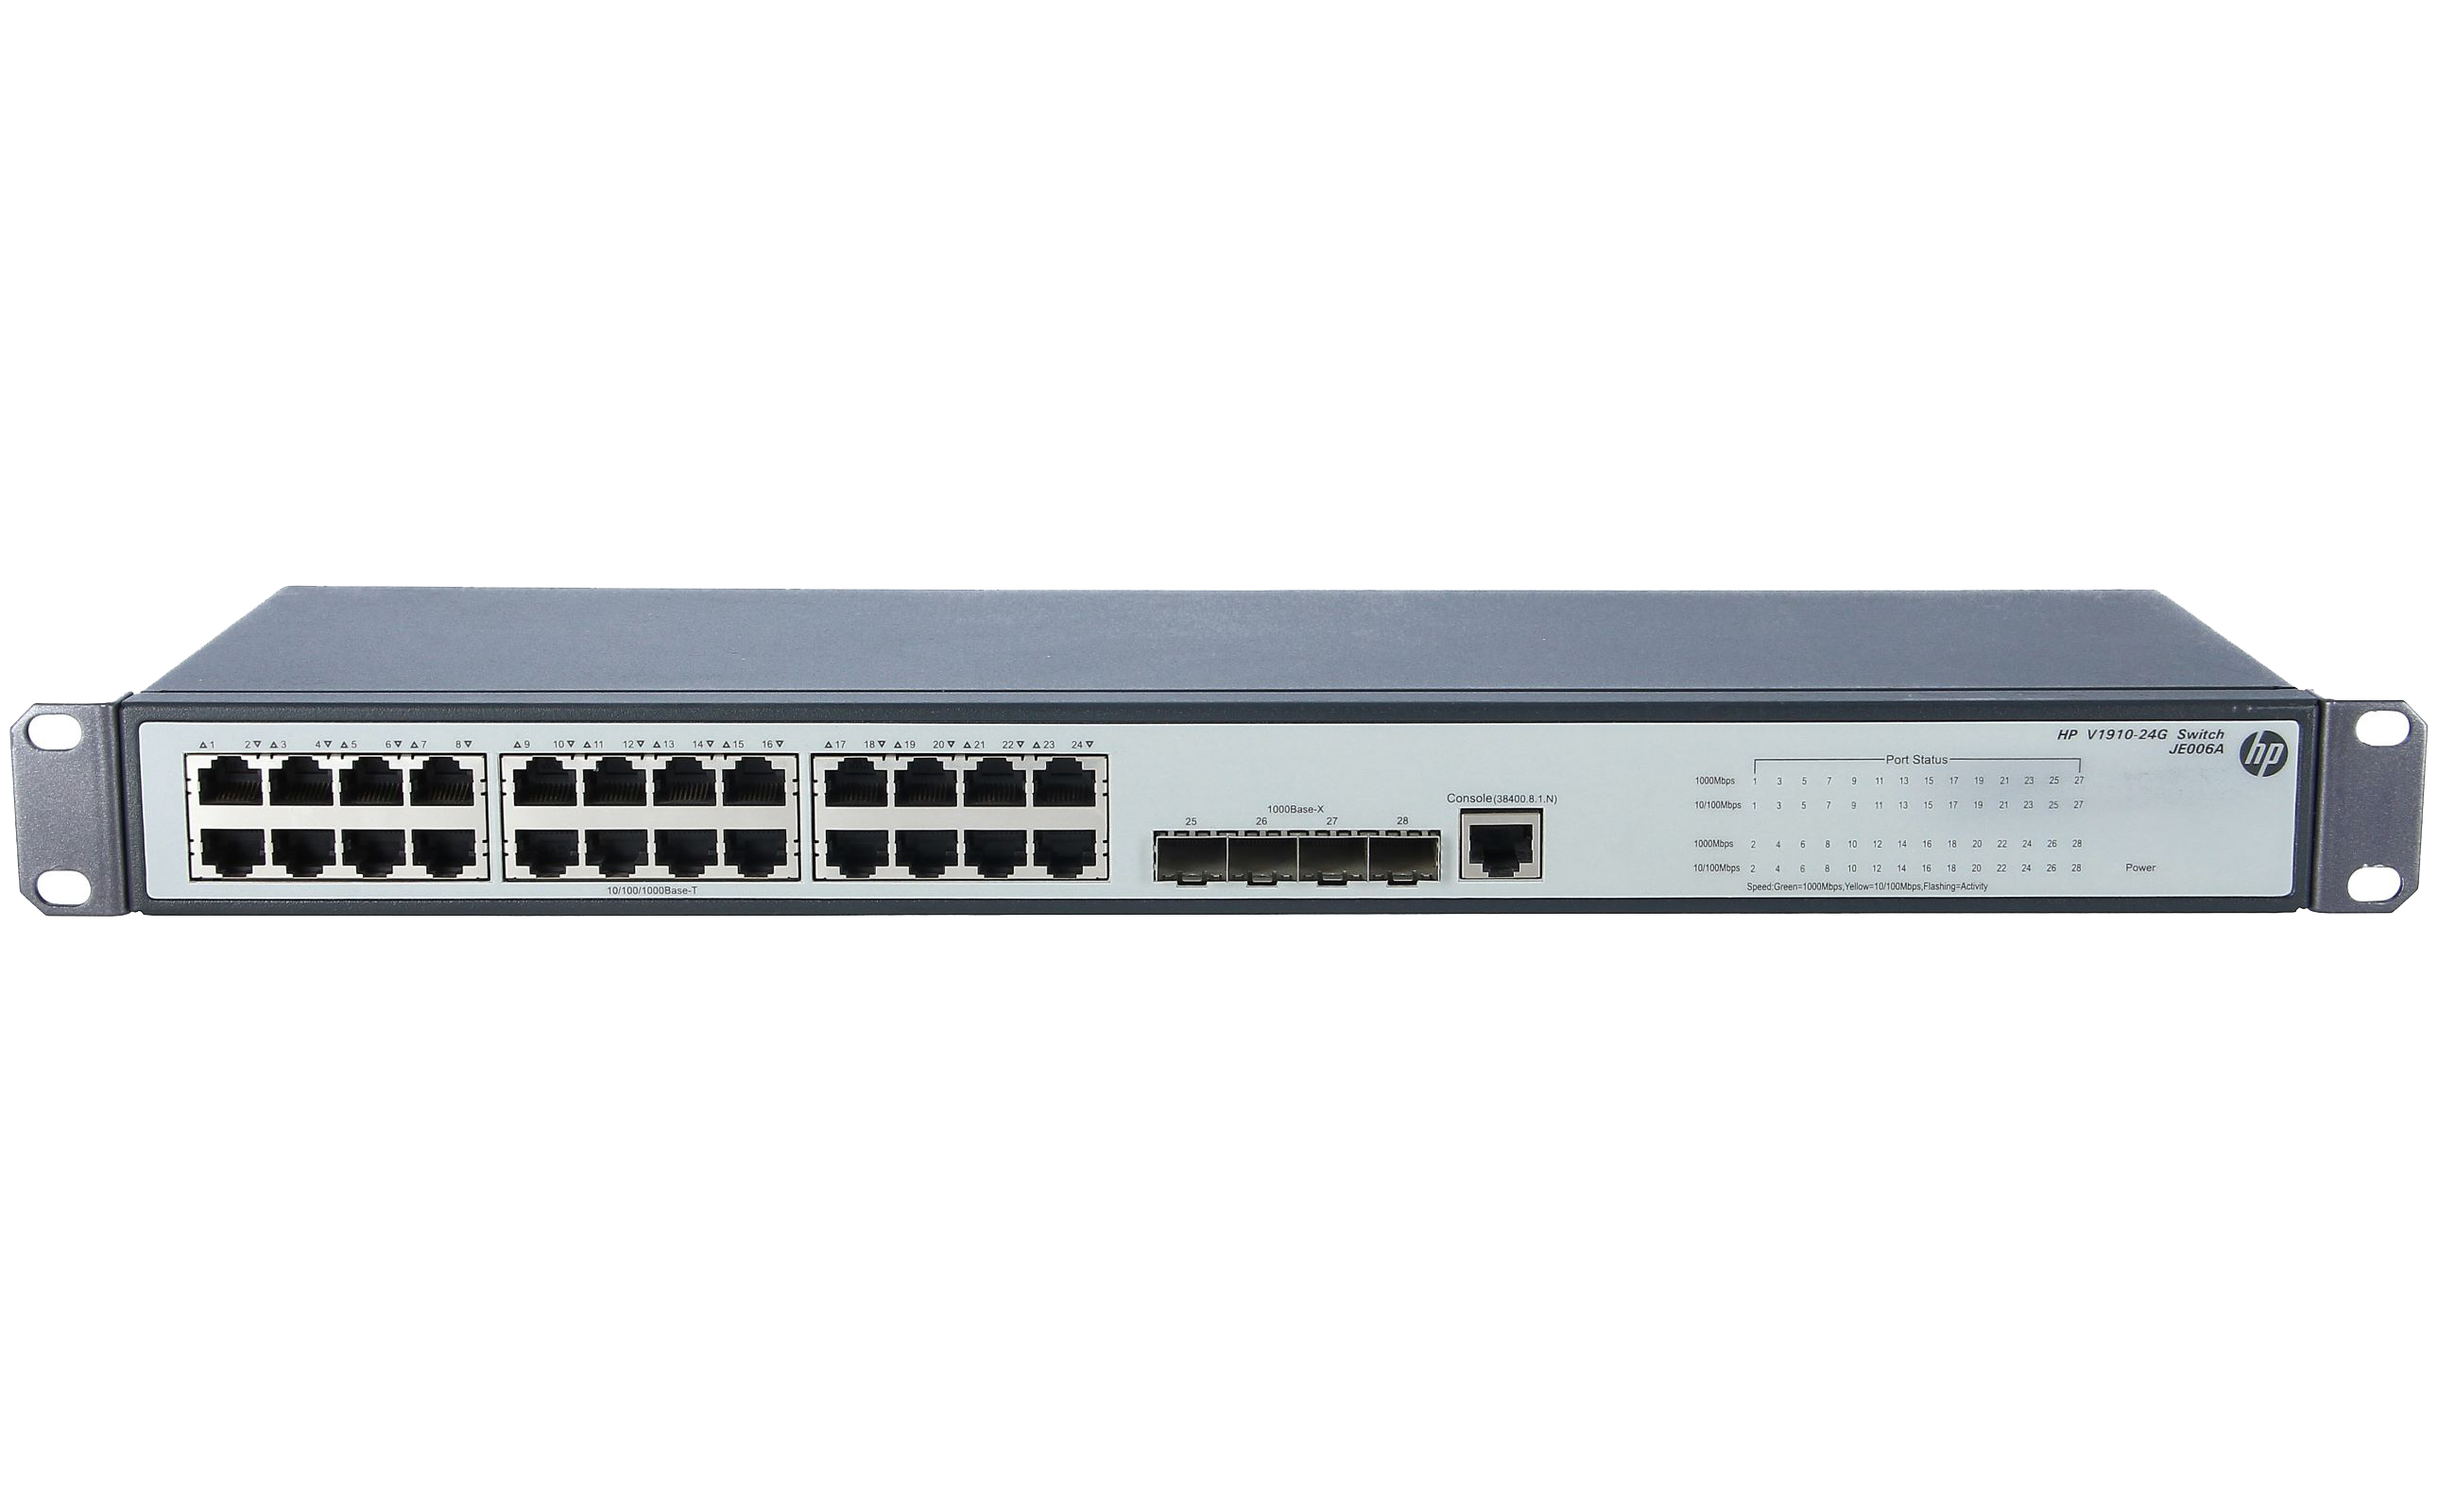
\includegraphics[width=3cm]{Images/HP1910.png} & Commutateurs HP1910 G24 & C'est un modèle de commutateur d'entreprise qui offre des fonctionnalités de gestion avancées pour les réseaux LAN. Il dispose de 24 ports Gigabit Ethernet et peut être géré via une interface web ou en ligne de commande. 

Il prend en charge les protocoles de gestion de réseau SNMP, RMON et LLDP, ainsi que les VLAN, le QoS, le STP et d'autres fonctionnalités de sécurité.  \\
\hline
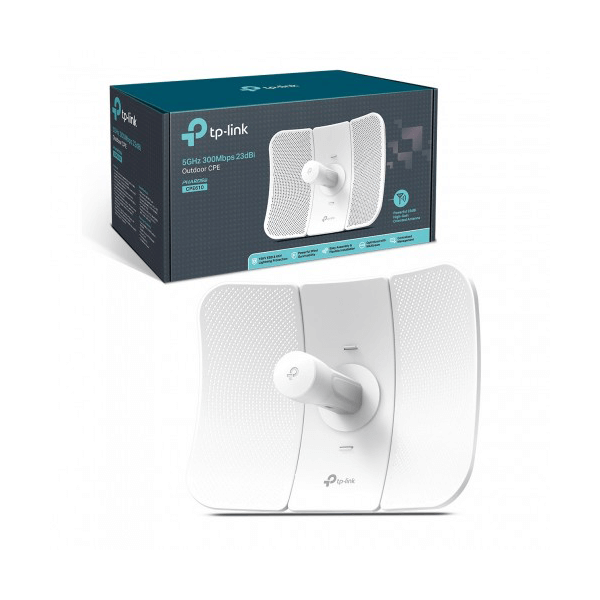
\includegraphics[width=3cm]{Images/TP-Link-CPE610-5GHz_1.png} & TP-Link CPE610 & Le TP-Link CPE610 est un point d'accès extérieur sans fil conçu pour fournir une connectivité Wi-Fi à longue portée dans des environnements extérieurs. 

Il utilise une antenne directionnelle à haut gain pour offrir des connexions sans fil stables et fiables sur de longues distances.  \\
\hline
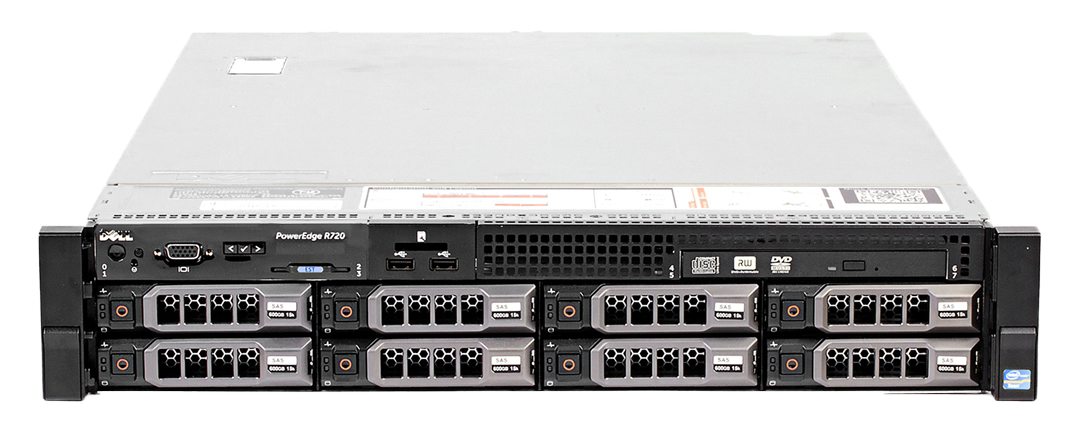
\includegraphics[width=3cm]{Images/dellr720.png} & Dell PowerEdge R720 & Le Dell PowerEdge R720 est un serveur rackable de haute performance, fiable et évolutif, offrant une grande capacité de stockage et de traitement de données pour les applications critiques de l'entreprise. 

Il est équipé de processeurs Intel Xeon E5-2600 v2 et peut prendre en charge jusqu'à 1,5 To de mémoire vive. Le PowerEdge R720 dispose également de fonctionnalités de haute disponibilité telles que les alimentations redondantes, les disques durs en miroir et les cartes réseau doubles. \\
\hline
\end{tabular}
\caption{Matériels utilisés}
\label{1}
\end{center}
\end{table}


\subsection{Logiciels utilisés}

Dans cette sous-section, nous présentons dans les tableaux \ref{2} et \ref{3} les logiciels utilisés comme les GNS3 et VNC Viewer dans notre projet pour créer notre infrastructure réseau. 


\begin{table}[H]
\begin{tabular}{|c{3cm}|c{3cm}|l{10cm}|}
\hline
\textbf{Logo}         & \textbf{Nom de l'équipement}   & \textbf{Fonctionnalité} \\
\hline

\includegraphics[width=3cm]{Images/Logo-GNS3.png} & GNS3 & GNS3 est un logiciel open-source de simulation de réseaux informatiques. 

Il permet de créer des topologies réseau virtuelles en utilisant des images de routeurs, de commutateurs et d'autres équipements réseau. \\
\hline

\includegraphics[width=3cm]{Images/Logo-VMWare.jpg}  & VMware Workstation & VMware Workstation est un logiciel de virtualisation puissant qui permet d'exécuter plusieurs systèmes d'exploitation sur une seule machine physique. 

Il offre la possibilité de créer et de gérer des machines virtuelles (VM) sur une plateforme hôte, ce qui permet d'exécuter plusieurs systèmes d'exploitation simultanément. VMware Workstation est disponible pour les principales plateformes telles que Windows, Linux et macOS. \\
\hline

\includegraphics[width=3cm]{Images/Logo-VNCViewer.png} & VNC Viewer & VNC Viewer est une application de bureau à distance qui permet de se connecter à un ordinateur distant et d'en contrôler l'écran et les applications à distance. 

Il offre la possibilité de se connecter à distance à des appareils tels que le Raspberry Pi, permettant ainsi une gestion et un contrôle pratiques de l'appareil à partir d'un autre ordinateur. \\
\hline

\includegraphics[width=3cm]{Images/Logo-IPScanner.png} & Advanced IP Scanner & Advanced IP Scanner est un outil de gestion de réseau qui permet de scanner rapidement un réseau et de trouver tous les périphériques connectés, y compris les ordinateurs, les imprimantes, les routeurs, les commutateurs, les caméras IP, etc.

Il permet également de détecter les adresses IP inactives et les ports ouverts sur les périphériques.  \\
\hline
\end{tabular}
\caption{Logiciels utilisés}
\label{2}
\end{table}


\begin{table}[H]
\begin{center}
\begin{tabular}{|c{3cm}|c{3cm}|l{10cm}|}
\hline

\includegraphics[width=3cm]{Images/Logo-Fritzing.png} & Fritzing & Fritzing est un logiciel de conception électronique open-source qui permet de créer des schémas électroniques, des circuits imprimés et des modèles de connexion pour des projets électroniques. 

Il offre une interface conviviale et intuitive, ce qui facilite la création de schémas électroniques même pour les débutants. \\
\hline
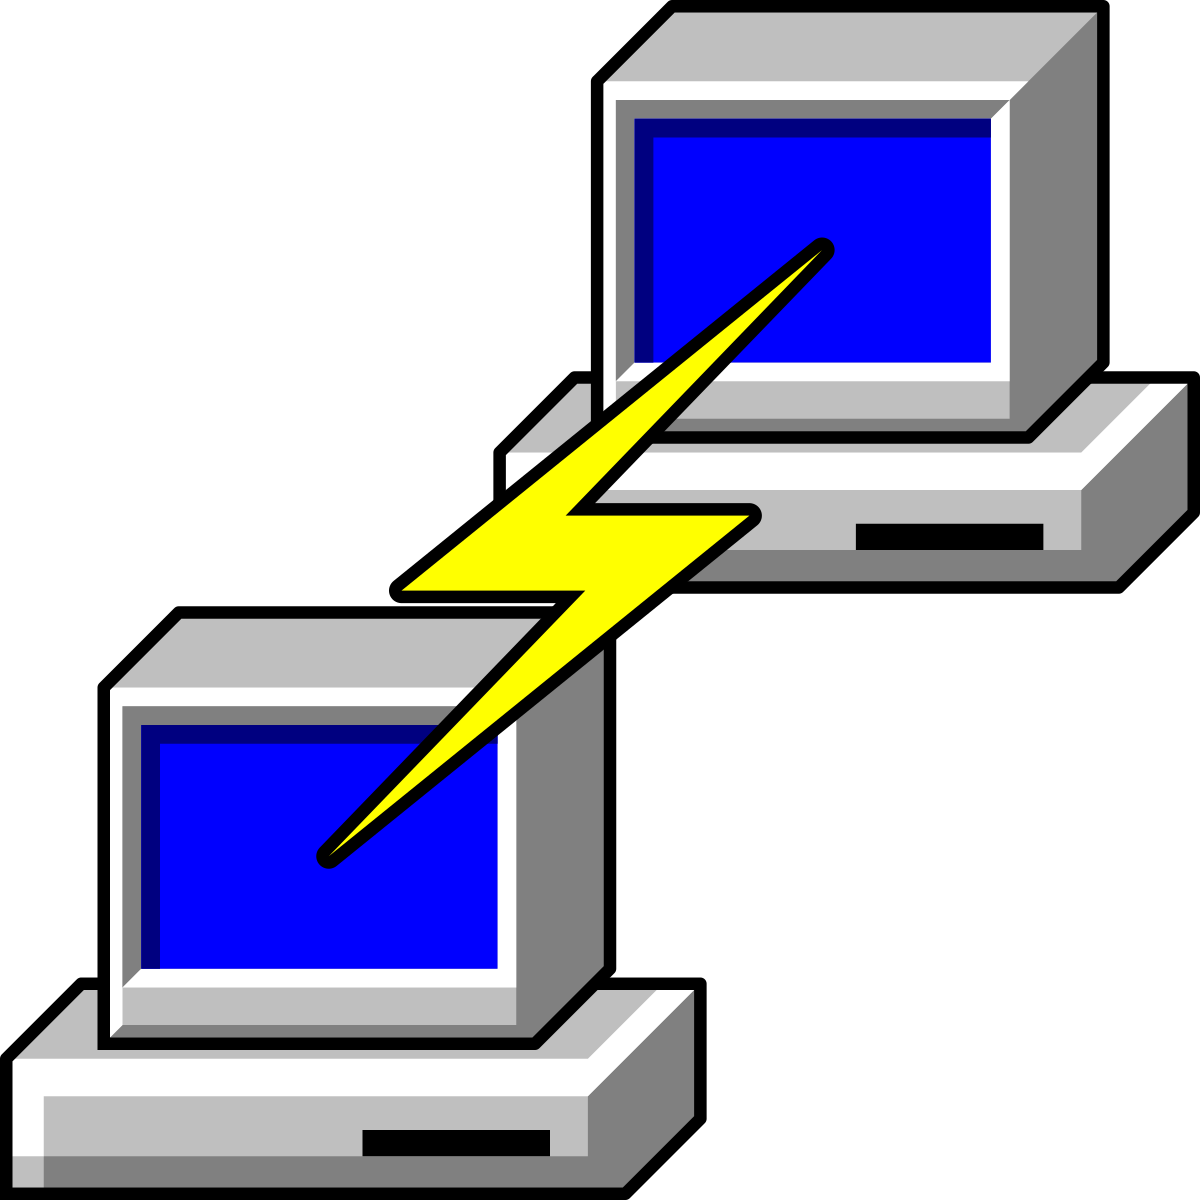
\includegraphics[width=3cm]{Images/Logo-Putty.png} & Putty & PuTTY est un logiciel client pour les protocoles de communication SSH, Telnet et Rlogin, permettant d'établir des connexions réseau sécurisées avec des ordinateurs distants. 

Il est utilisé principalement pour administrer des serveurs à distance, mais peut également être utilisé pour des transferts de fichiers et des sessions de console distantes. \\
\hline

\includegraphics[width=3cm]{Images/Logo-Raspberry.png} & Raspberry Pi Imager & Raspberry Pi Imager est un logiciel qui permet de facilement installer des systèmes d'exploitation sur une carte SD ou une clé USB pour Raspberry Pi. 

Il offre une interface graphique simple à utiliser pour sélectionner et télécharger les images d'OS disponibles. \\
\hline

\includegraphics[width=3cm]{Images/xminglogo.png} & Xming & Xming est un serveur d'affichage X open source qui permet d'exécuter des applications graphiques Linux sur des systèmes Windows. 

Il fournit un environnement graphique pour les applications Linux, ce qui permet aux utilisateurs de Windows d'accéder et d'interagir avec des applications Linux à distance. \\
\hline
\end{tabular}
\caption{Logiciels utilisés - Suite}
\label{3}
\end{center}
\end{table}


\section{Présentation des locaux et déploiement de réseaux MAN}

Cette section nous plongeons au cœur de nos installations et de notre infrastructure de réseau métropolitain (MAN). Nous débutons par une présentation détaillée de nos trois locaux, chacun ayant ses caractéristiques uniques. Ensuite, nous explorons la notion de réseau MAN et son importance pour notre entreprise. Enfin, nous dévoilons les coulisses de l'implémentation de notre MAN, en mettant en lumière nos choix stratégiques, notamment notre préférence pour les équipements TP-Link.




\subsection{Présentation des trois locaux}

Dans le cadre de notre projet de Mémoire de Mastère, nous avons été accueillis au sein de Zeta Engineering. Cette entreprise, établie en Tunisie, dispose de trois nouveaux locaux distincts, chacun jouant un rôle essentiel dans ses opérations.

Le premier local, situé à Rades Meliane, Rue de la Solidarité, est principalement réservé à l'administration de l'entreprise et à l'équipe chargée de la diffusion globale. Il s'agit d'un espace central pour la gestion des activités quotidiennes de l'entreprise et la coordination de ses opérations à l'échelle nationale et internationale. C'est également le local le plus important en termes de sécurité, c'est pourquoi nous y installons un Pare-Feu dédié. 

Le deuxième local, situé à Rades, Rue Habib Bourgiba, abrite le centre d'appel de Zeta Engineering. C'est ici que l'équipe prend en charge les appels des clients, traite leurs demandes et fournit un support essentiel pour la clientèle. Nous avons donc besoin principalement d'une connexion Internet par fibre optique fiable, c'est pourquoi nous installons un routeur Cisco à cet endroit.

Enfin, le troisième local, situé à Ezzahra, Rue Habib Bourgiba, est l'espace de travail pour les ingénieurs et les développeurs informatiques de l'entreprise. C'est dans cet espace que les produits technologiques de Zeta Engineering sont conçus et développés.

Ces deux figures \ref{Chap2.4.21} et figure \ref{Chap2.5.5} ci-dessous montrent la distance entre le bureau Rades Meliane et le bureau Rades, qui est d'environ 1,268 km, ainsi que la distance entre le bureau Rades Meliane et Ezzahra, qui est d'environ 2,843 km.

\begin{figure}[H]
\centering
\includegraphics[width=16cm]{Images/distance1.png}
\caption{Distance entre le bureau Rades et Rades Meliane (1,268 km)}
\label{Chap2.4.21}
\end{figure}


\begin{figure}[H]
 \centering
    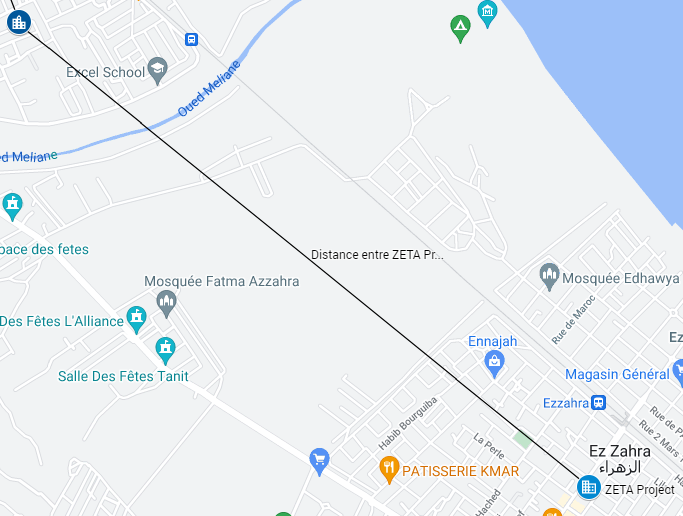
\includegraphics[width=16cm]{Images/Distance2.png}
    \caption{Distance entre bureau Rades et bureau Ezzhara (2,843 km)}
    \label{Chap2.5.5}
\end{figure}    

Avec ces trois locaux répartis géographiquement, comme le montre la figure \ref{Chap2.6.0}, il devient essentiel de mettre en place un réseau de zone métropolitaine (MAN) pour les connecter de manière transparente. 

Un réseau MAN permettra à Zeta Engineering de relier ses bureaux de Rades Habib Bourgiba, Rades Meliane et Ezzahra, garantissant ainsi une communication fluide et efficace entre eux.

\begin{figure}[H]
\centering
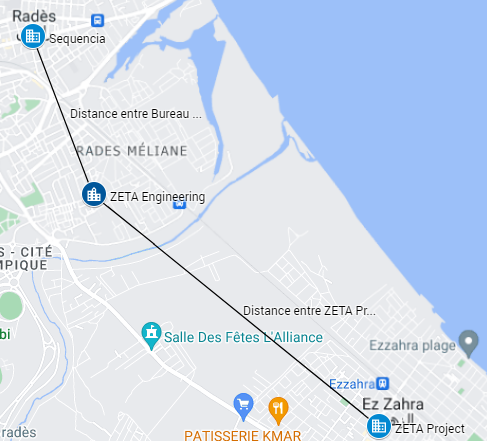
\includegraphics[width=16cm]{Images/DistanceTotal.png}
\caption{Distance totale entre les bureaux}
\label{Chap2.6.0}
\end{figure}

Ce réseau joue un rôle crucial dans la centralisation des données, la gestion des ressources et la coordination des activités à l'échelle de l'entreprise. De plus, il intègre également les objets connectés tels que les machines de pointage, les capteurs de température et d'humidité, les lampes, les smartphones et les caméras de surveillance, optimisant ainsi l'utilisation de ces ressources au sein de l'entreprise. 

En fin de compte, le réseau MAN contribue à renforcer l'efficacité opérationnelle de Zeta Engineering et répond aux besoins croissants du marché et de la technologie.


\subsection{Définition du réseau MAN}

Un réseau MAN est un type de réseau de communication qui couvre une zone géographique intermédiaire entre un réseau LAN et un réseau WAN \cite{sze1985metropolitan}. 


\begin{figure}[H]
 \centering
    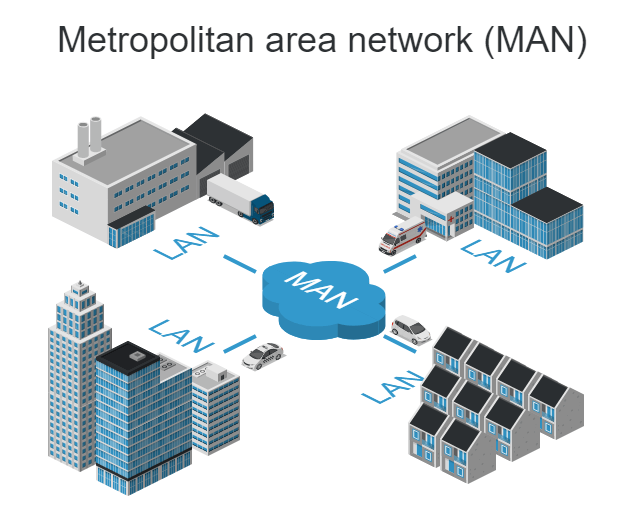
\includegraphics[width=15cm]{Images/network-man1.png}
    \caption{Metropolitan Area Network}
    \label{Chap2.3.1}
\end{figure}  

Contrairement à un réseau LAN qui est généralement limité à une seule installation ou à un seul site comme démontré dans la figure \ref{Chap2.3.1}, un réseau MAN s'étend sur une zone géographique plus étendue, comme une ville entière ou une zone métropolitaine. 


Dans le contexte de notre projet à Zeta Engineering, l'objectif est de relier les trois bureaux de l'entreprise situés à Rades Habib Bourgiba, Rades Meliane et Ezzahra via un réseau MAN pour permettre une communication efficace et une gestion centralisée des ressources. 


\subsection{Implémentation du MAN et le choix de TP-Link}

Pour établir notre réseau étendu (MAN), nous choisissons  d'utiliser le TP-Link CPE610. Ce point d'accès sans fil est spécialement conçu pour offrir une connectivité longue distance en utilisant la fréquence de 5 GHz.

Nous suivons les étapes d'assemblage et d'installation illustrées dans les figures \ref{Chap2.3.2} et \ref{Chap2.3.4} ci-dessous pour installer le TP-Link CPE610.

\begin{figure}[H]
\centering
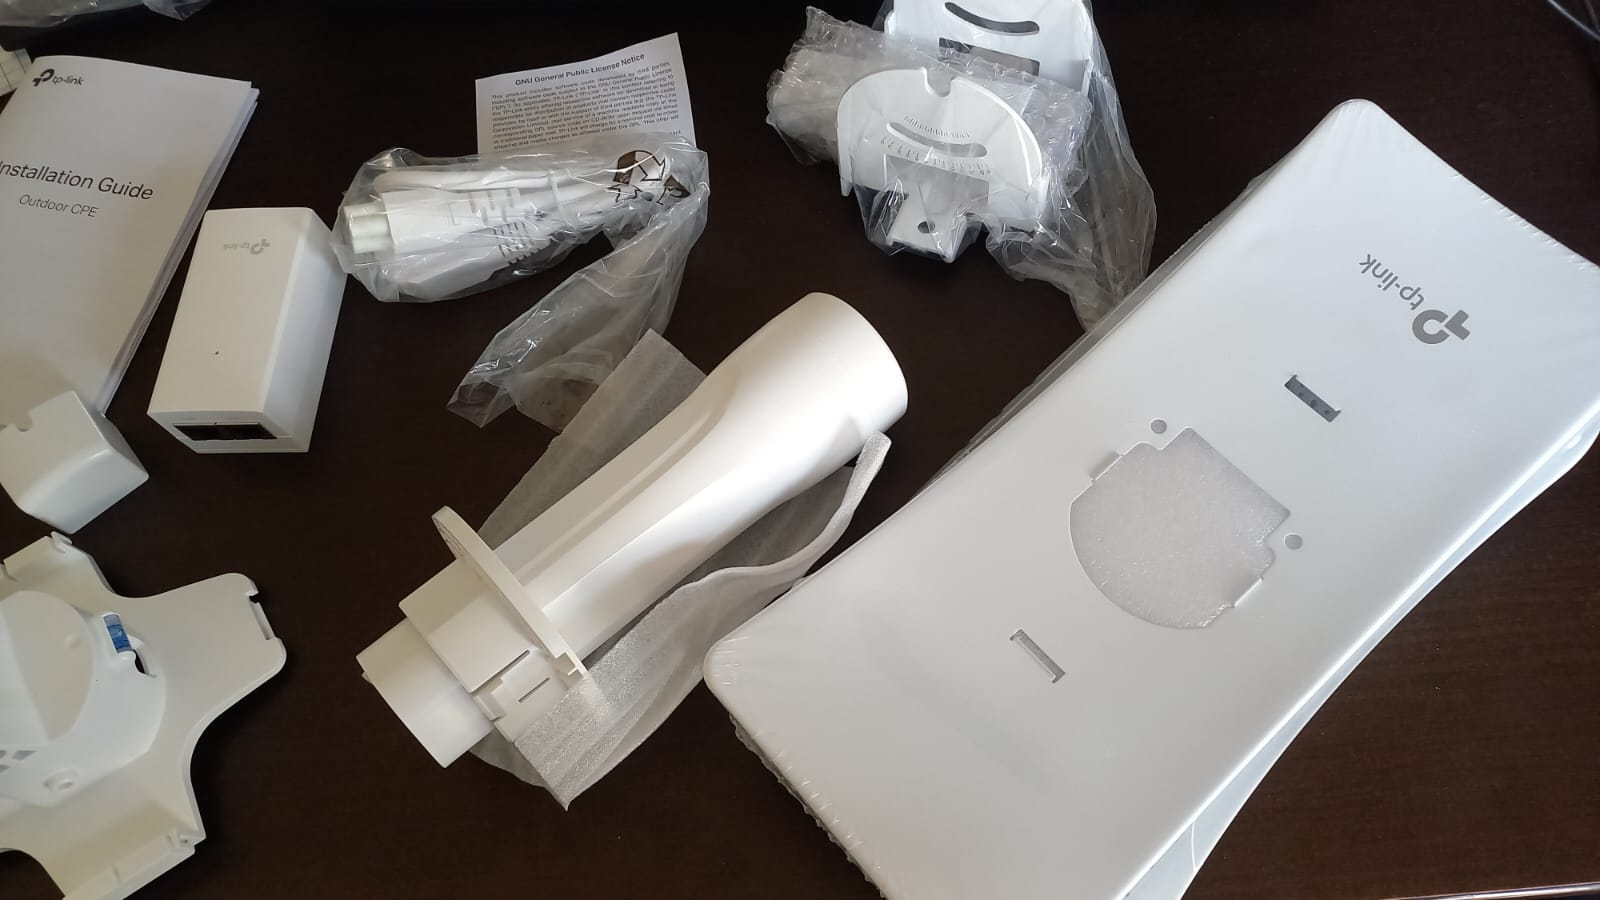
\includegraphics[width=15cm]{Images/SetupTPL4.jpg}
\caption{Déballage du TP-Link CPE610}
\label{Chap2.3.2}
\end{figure}

\begin{figure}[H]
\centering
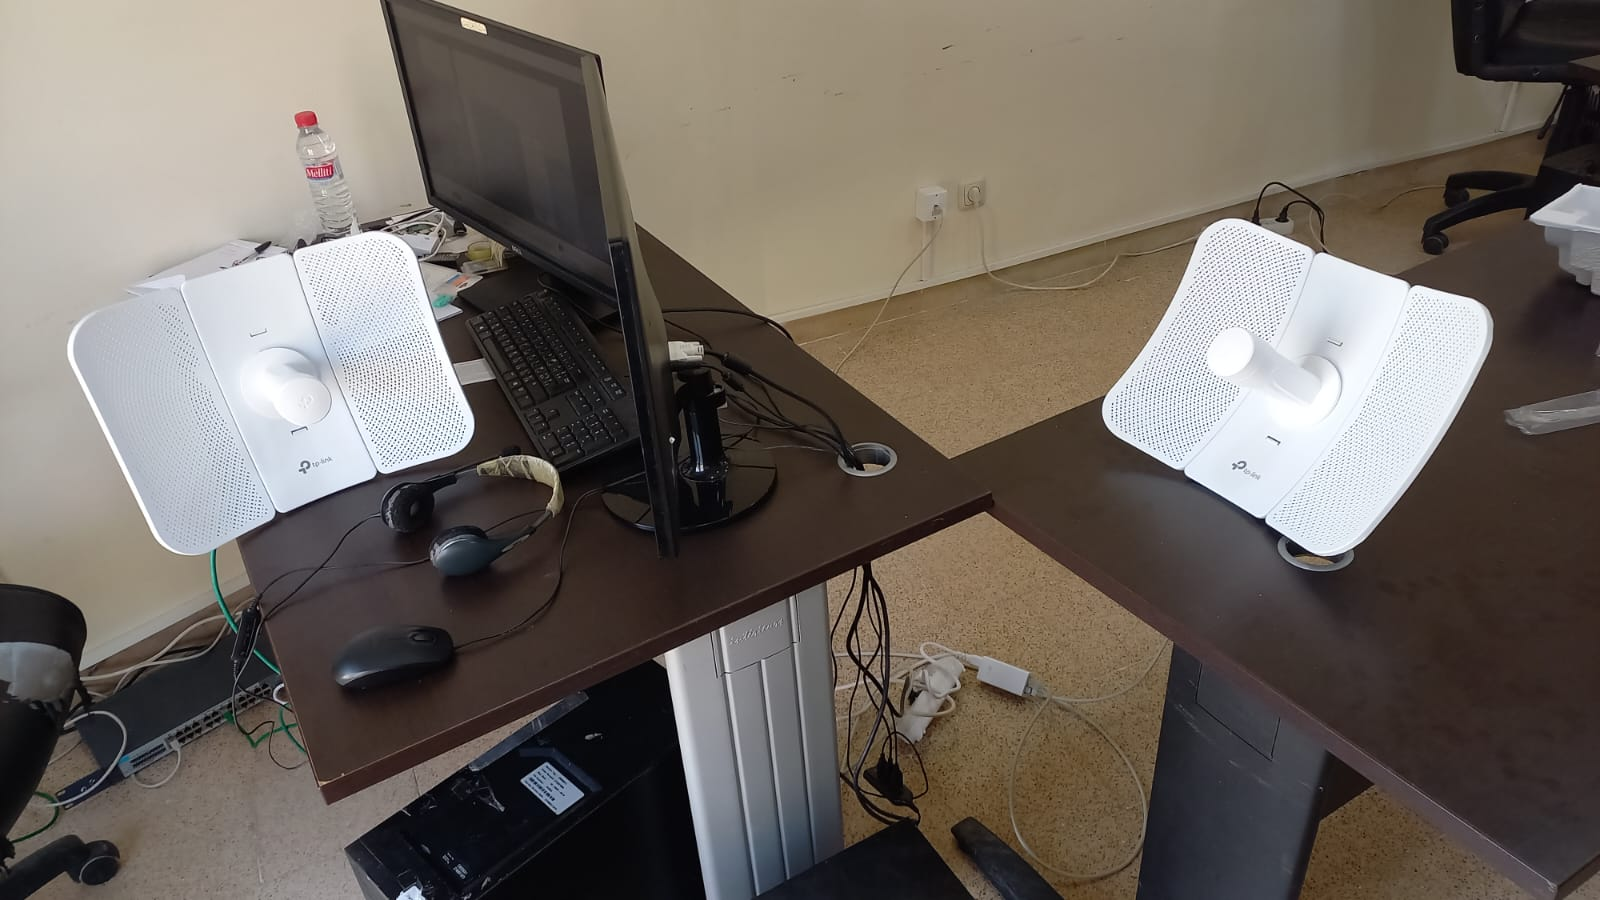
\includegraphics[width=15cm]{Images/SetupTPL1.jpg}
\caption{Assemblage des pièces du TP-Link CPE610}
\label{Chap2.3.4}
\end{figure}


Après avoir soigneusement assemblé les différentes composantes du TP-Link, nous sommes en mesure d'accéder à son panneau d'administration via une connexion LAN. À partir de là, nous entamons le processus d'initialisation et de configuration.

La figure \ref{Chap2.3.5} illustre l'étape d'initialisation du TP-Link, où nous configurons  les paramètres essentiels pour son bon fonctionnement.

\begin{figure}[H]
\centering
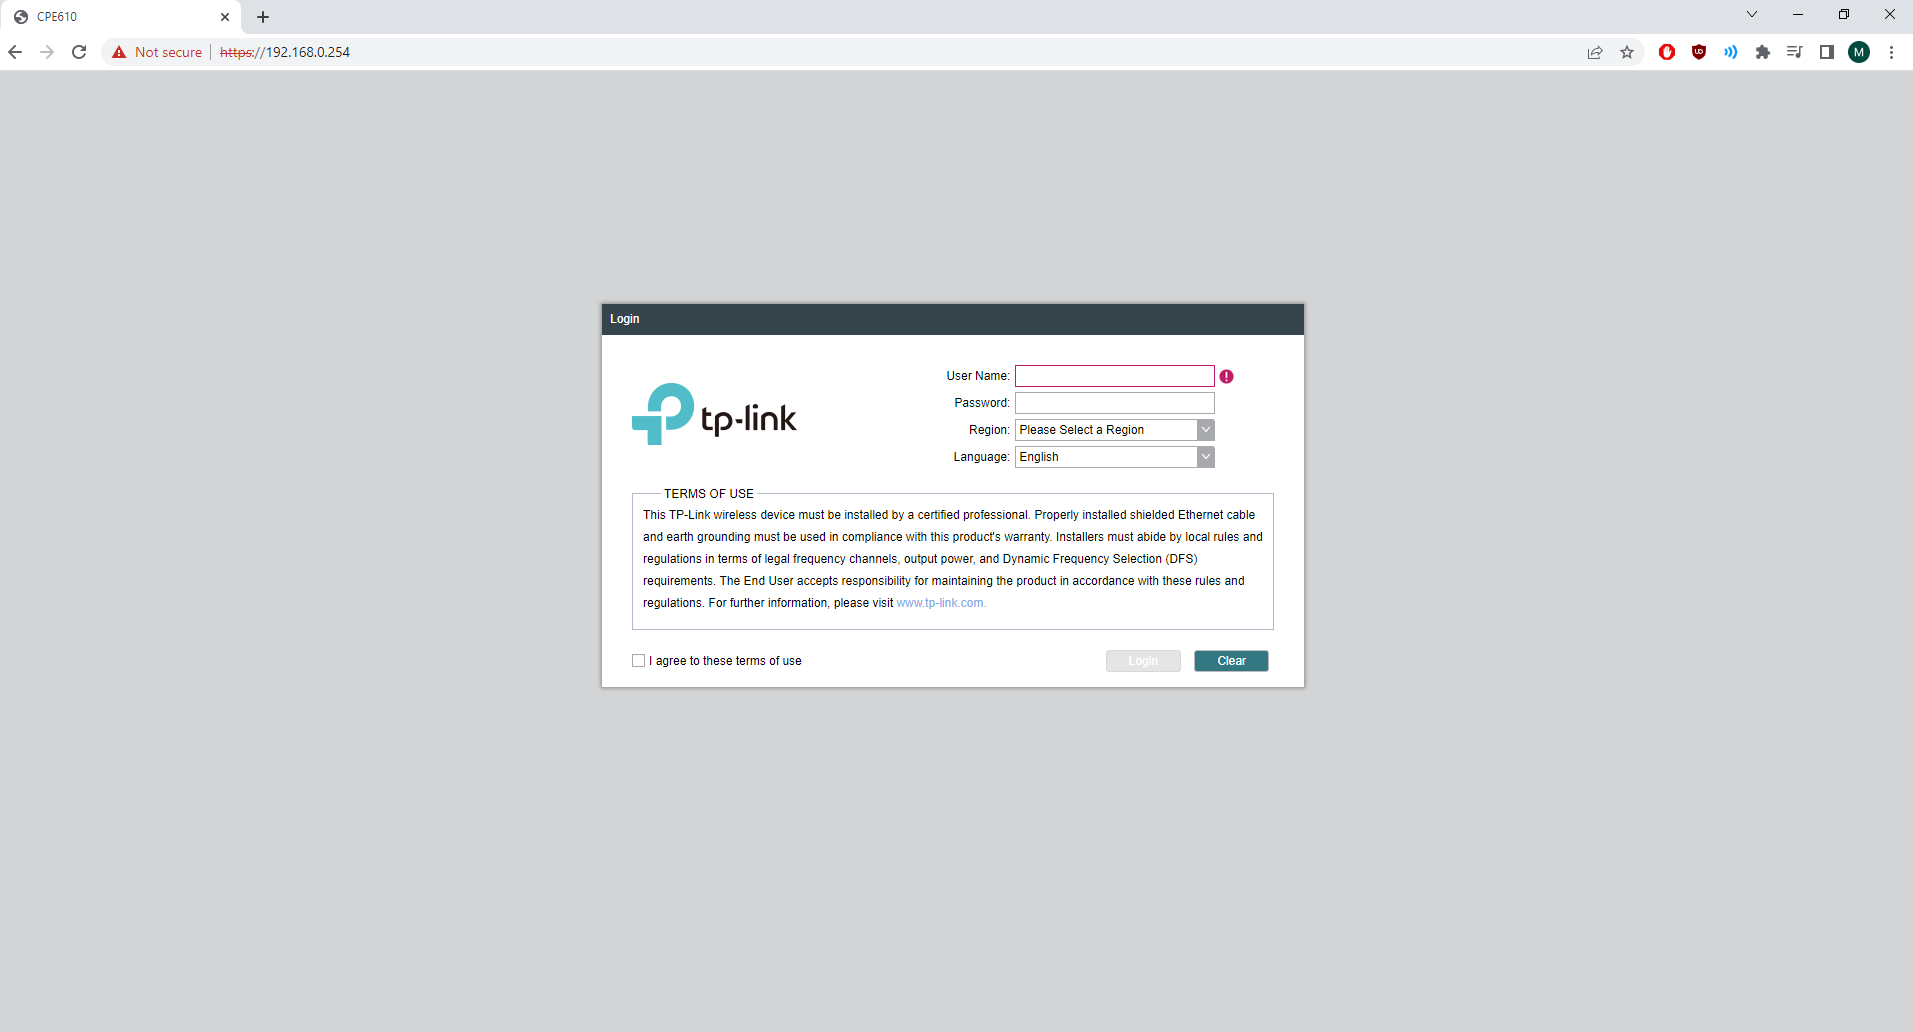
\includegraphics[width=15cm]{Images/tplink3.png}
\caption{Initialisation du TP-Link}
\label{Chap2.3.5}
\end{figure}

La configuration en mode test est représentée dans la figure \ref{Chap2.3.6}, nous permettant de vérifier les performances du dispositif avant une utilisation complète.

\begin{figure}[H]
\centering
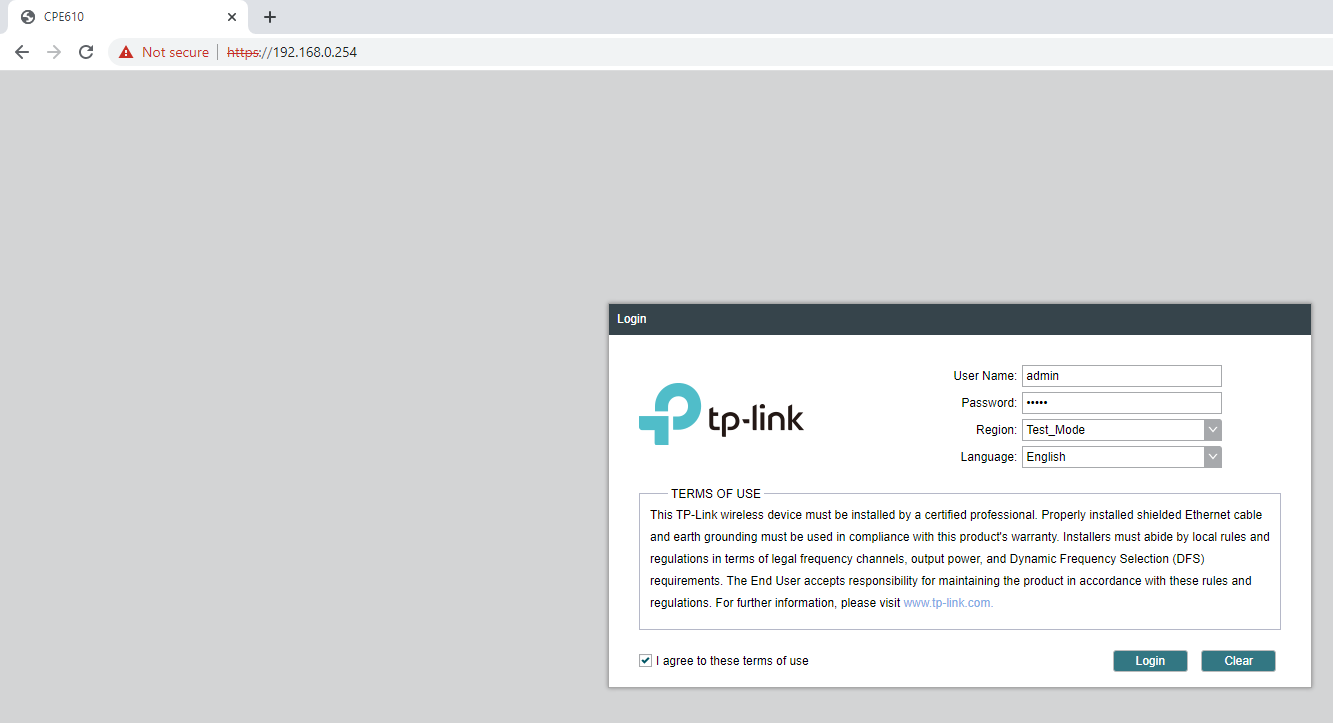
\includegraphics[width=15cm]{Images/tplink33.png}
\caption{Initialisation du TP-Link en mode test}
\label{Chap2.3.6}
\end{figure}

Le panneau de contrôle complet du TP-Link est dépeint dans la figure \ref{Chap2.3.7}, où nous pouvons régler et surveiller divers paramètres pour garantir un réseau stable.

\begin{figure}[H]
\centering
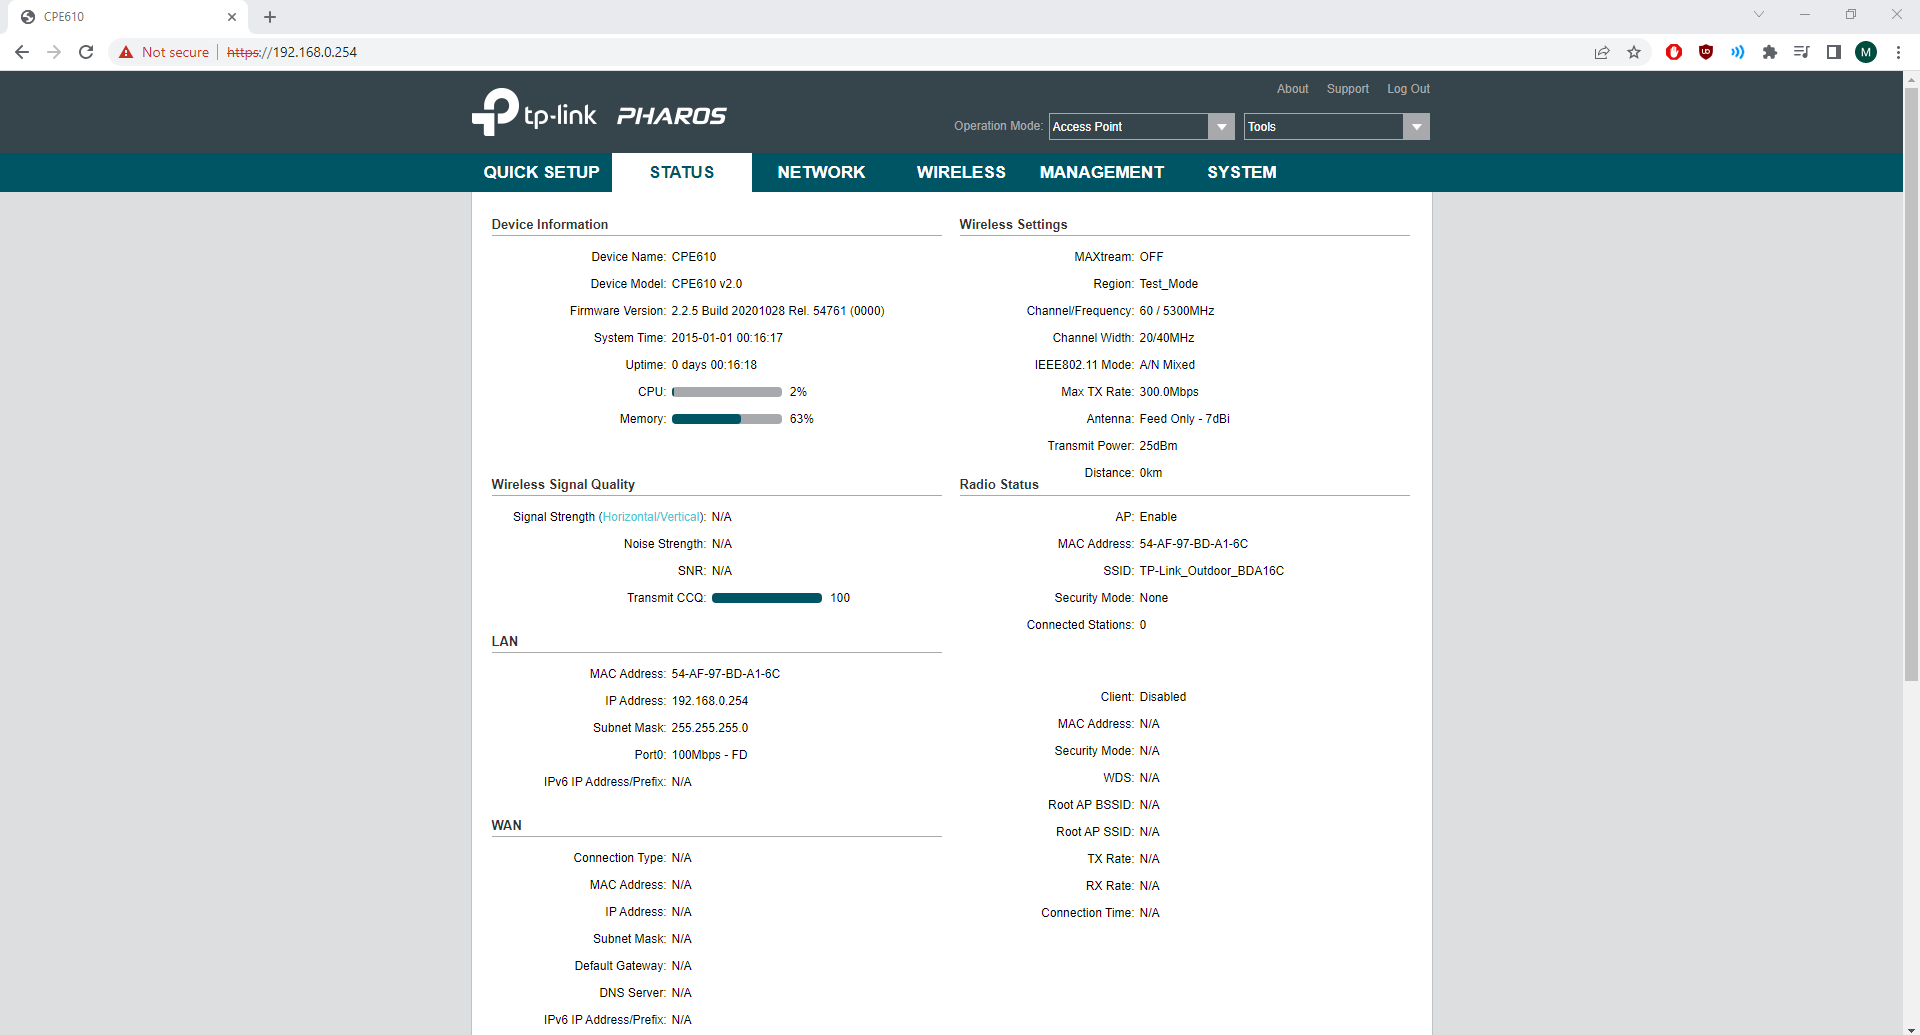
\includegraphics[width=15cm]{Images/tplink34.png}
\caption{Panneau de contrôle du TP-Link}
\label{Chap2.3.7}
\end{figure}

Les figures \ref{Chap2.3.8} et \ref{Chap2.3.9} montrent respectivement les étapes d'initialisation de l'émetteur et du récepteur du TP-Link, éléments clés pour établir une connexion fiable.

\begin{figure}[H]
\centering
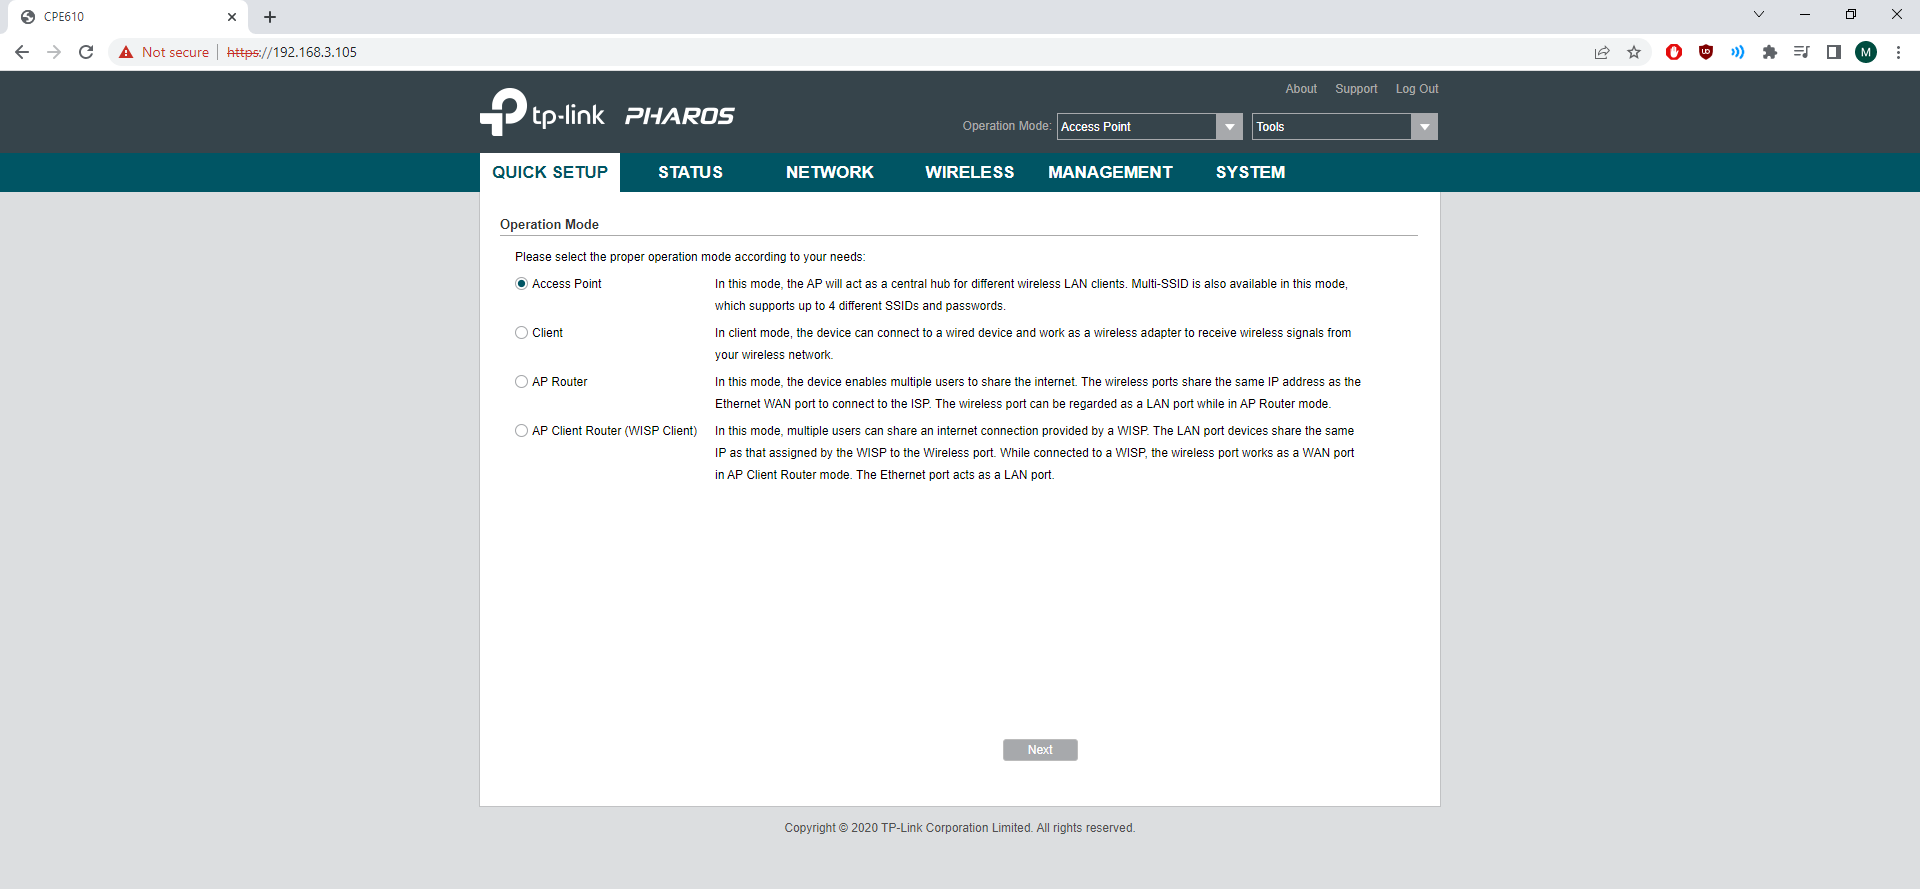
\includegraphics[width=15cm]{Images/tplink35.png}
\caption{Initialisation de l'émetteur}
\label{Chap2.3.8}
\end{figure}

\begin{figure}[H]
\centering
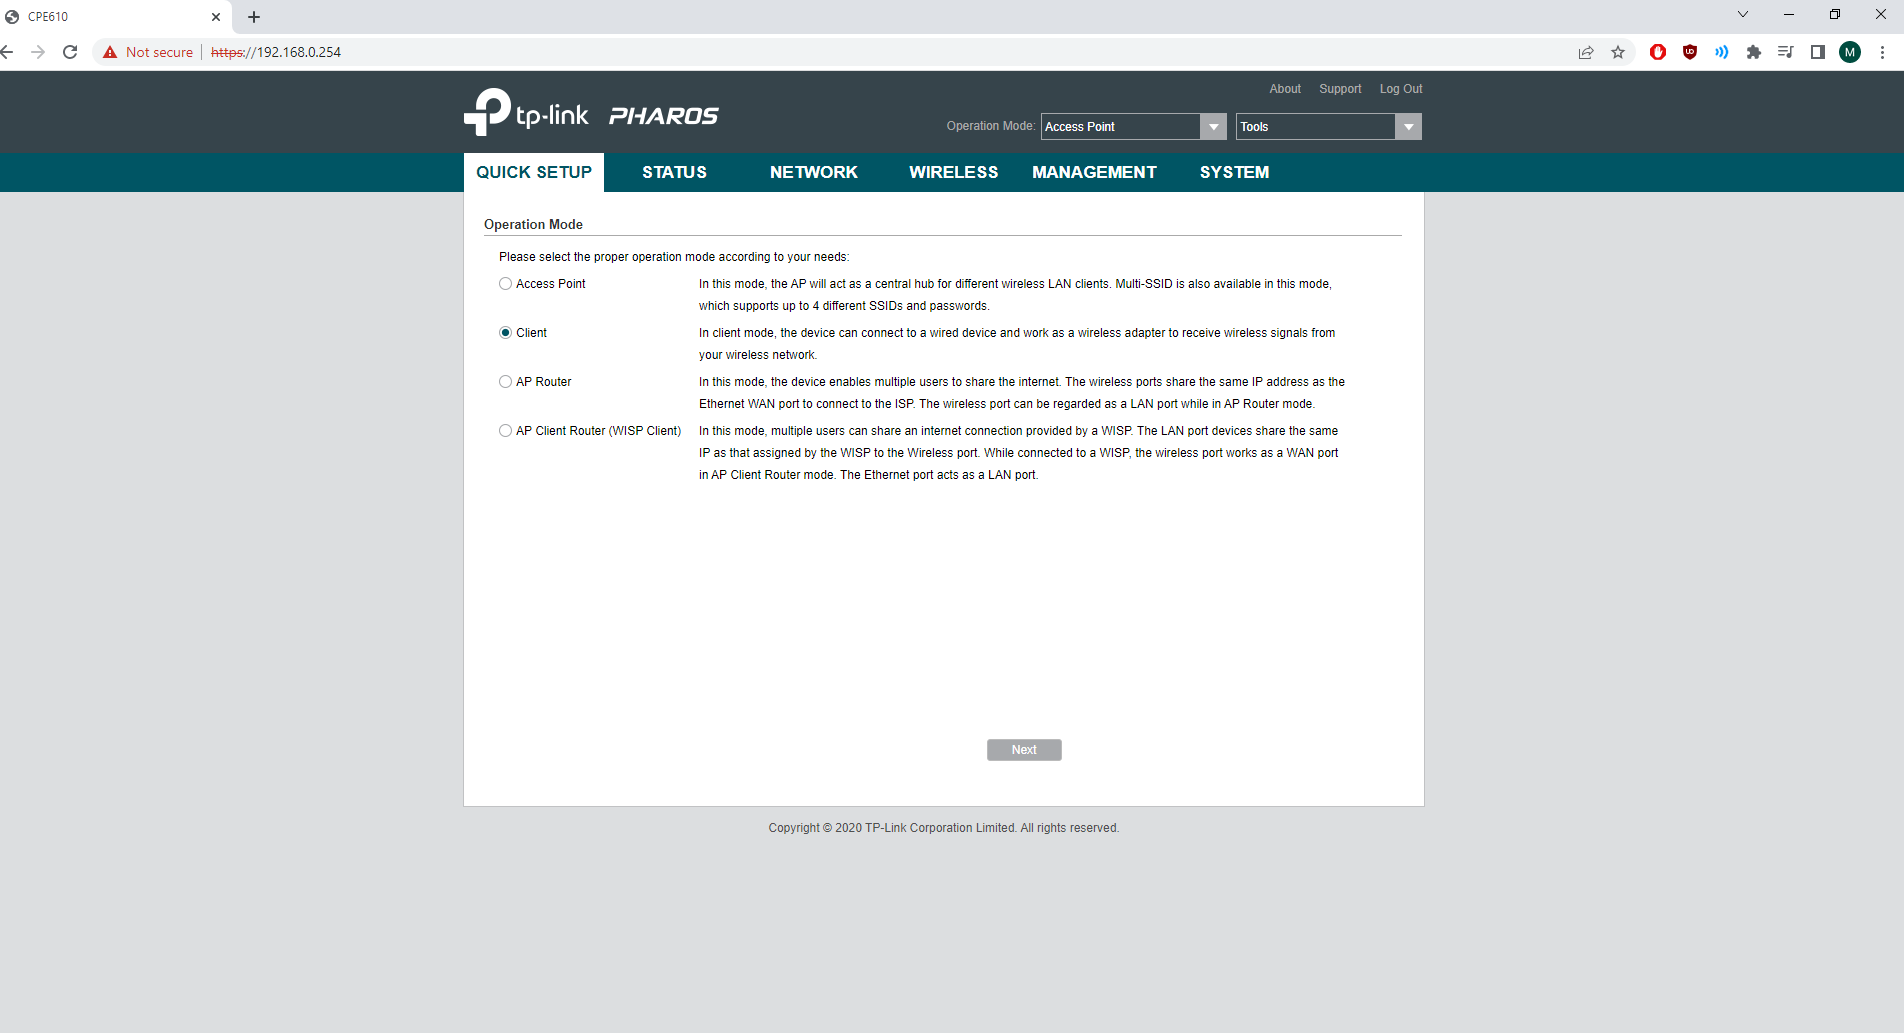
\includegraphics[width=15cm]{Images/tplink36.png}
\caption{Initialisation du récepteur}
\label{Chap2.3.9}
\end{figure}

L'étape finale de vérification de la connexion entre le point d'accès TP-Link et le client TP-Link est détaillée dans la figure et \ref{Chap2.3.11}.


\begin{figure}[H]
\centering
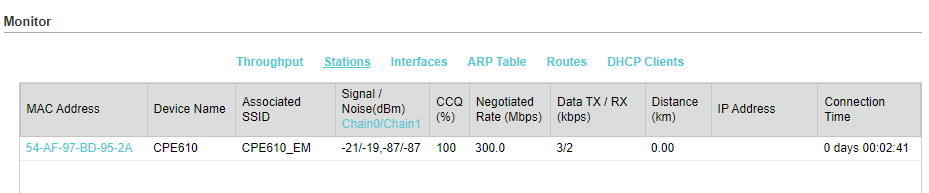
\includegraphics[width=15cm]{Images/TPLink4.png}
\caption{Test de connexion entre le point d'accès TP-Link et le client TP-Link}
\label{Chap2.3.11}
\end{figure}

Enfin, la figure \ref{Chap2.3.12} met en évidence l'installation réussie du TP-Link CPE610 à Rades Melian, marquant une étape cruciale de notre déploiement.

\begin{figure}[H]
\centering
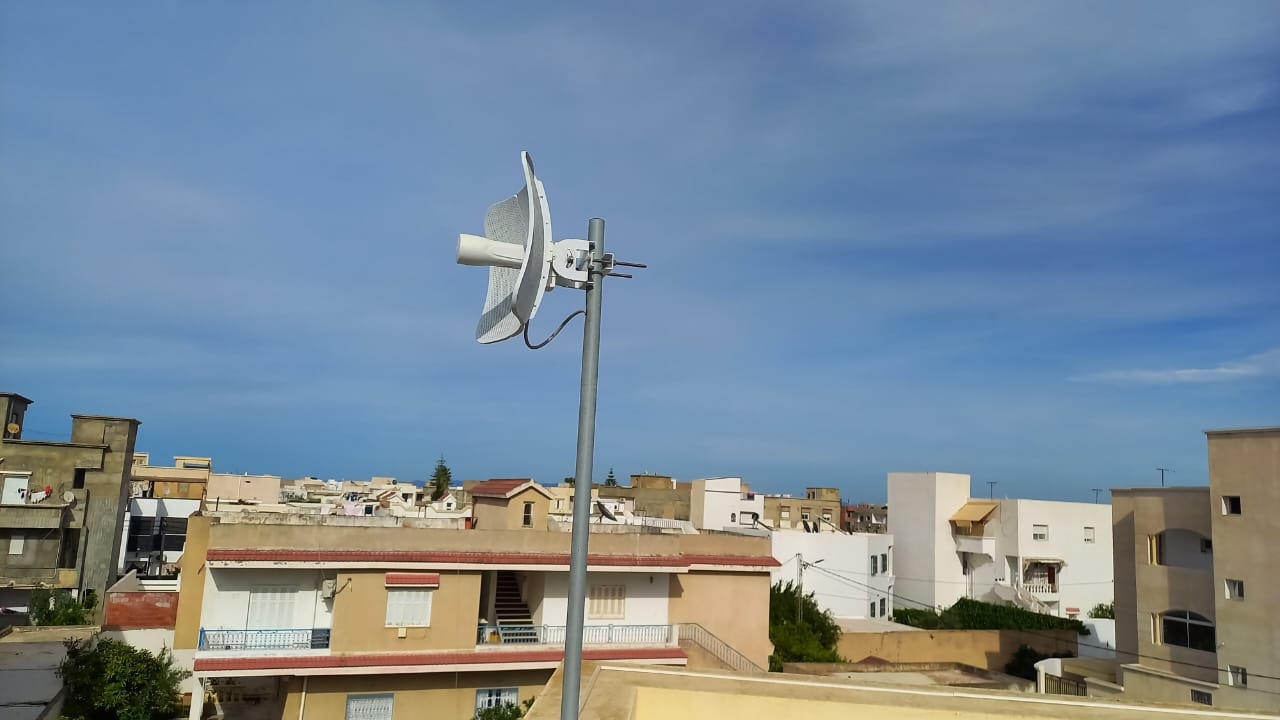
\includegraphics[width=15cm]{Images/BRadesMelian-TPLinkCEP610-1.jpeg}
\caption{Installation du TP-Link CPE610 à Rades Melian}
\label{Chap2.3.12}
\end{figure}

En suivant ces étapes, nous avons réussi à tester nos TP-Link et nous allons maintenant procéder à leur installation dans les différents bureaux.

\section{L'architecture réseau}

Dans cette section, nous plongeons au cœur de l'infrastructure qui soutient notre entreprise. Nous explorons en détail l'architecture réseau qui forme le socle de nos opérations. 

De la topologie de nos bureaux aux configurations dans GNS3 et à la mise en œuvre de notre infrastructure, cette section dévoile les coulisses de notre système de communication et de connectivité.


\subsection{Topologie en GNS3}


Dans cette section, nous présentons l'architecture réseau de chaque bureau à l'aide de simulations réalisées dans GNS3. L'objectif principal de ces simulations est de mettre en évidence l'efficacité de l'architecture réseau de chaque bureau, tout en nous permettant de démontrer la performance et la fiabilité de notre infrastructure. 

Cette approche nous a également donné l'opportunité d'anticiper et de résoudre d'éventuels problèmes avant qu'ils ne se manifestent dans le réseau réel, en effectuant des ajustements aux paramètres de configuration et en ajoutant de nouveaux équipements au besoin.

Pour commencer, nous modélisons les différents équipements du réseau de Rades, comme illustré dans la figure \ref{Chap2.2.0}. Le routeur C891F, par exemple, distribue l'accès Internet reçu de Topnet vers le commutateur principal HP-1910-G24. À partir de ce commutateur, nous gérons l'accès à Internet pour les utilisateurs et les connectons aux serveurs de la société.

\begin{figure}[H]
\centering
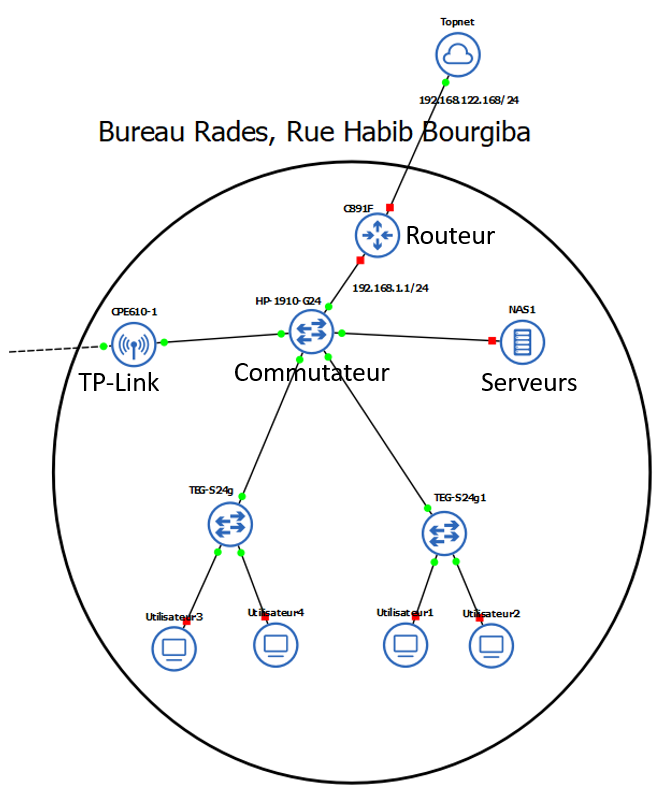
\includegraphics[width=16cm]{Images/BRades-Topologie.png}
\caption{Topologie du réseau du bureau de Rades}
\label{Chap2.2.0}
\end{figure}

Ensuite, dans la figure \ref{Chap2.4.1} nous présentons la topologie du réseau du bureau de Rades Meliane où nous remarquons que cette structure est similaire à celle mise en place dans le bureau de Rades, à la différence que nous ajoutons pfSense pour renforcer la sécurité du réseau principal vu que c'est le local le plus important assurant la gestion des activités quotidiennes de l'entreprise et la coordination de ses opérations à l'échelle nationale et internationale.

\begin{figure}[H]
\centering
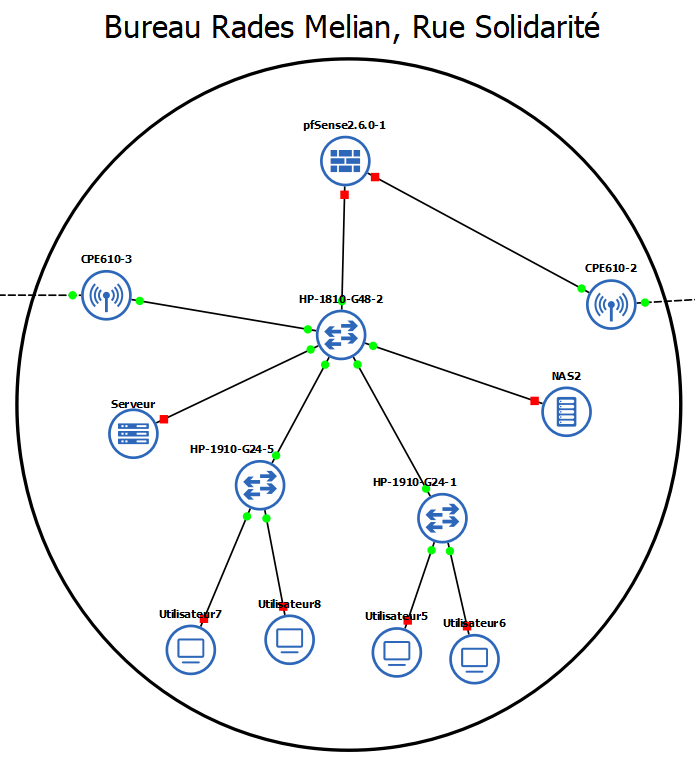
\includegraphics[width=15cm]{Images/BRadesMelian-Topologie.png}
\caption{Topologie du réseau du bureau de Rades Melian}
\label{Chap2.4.1}
\end{figure}

Enfin dans la figure \ref{Chap2.5.1}, pour le bureau Ezzahara nous ajoutons une source Internet supplémentaire à notre réseau au cas où l'accès Internet de Rades serait coupé ou interrompu.

\begin{figure}[H]
\centering
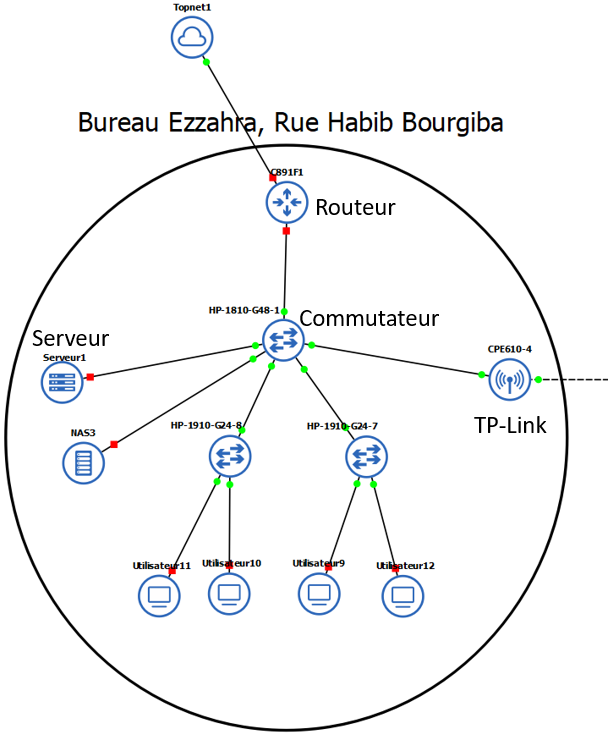
\includegraphics[width=15cm]{Images/BEzzahra-Topologie.png}
\caption{Topologie du réseau du bureau Ezzahara}
\label{Chap2.5.1}
\end{figure}



\subsection{Configuration en GNS3}

Dans cette section, nous présentons la configuration de notre réseau en utilisant GNS3. Tout d'abord, nous montrons la topologie du réseau dans la figure \ref{Chap2.2.1}, où nous avons accès à la console du routeur. 


\begin{figure}[H]
 \centering
    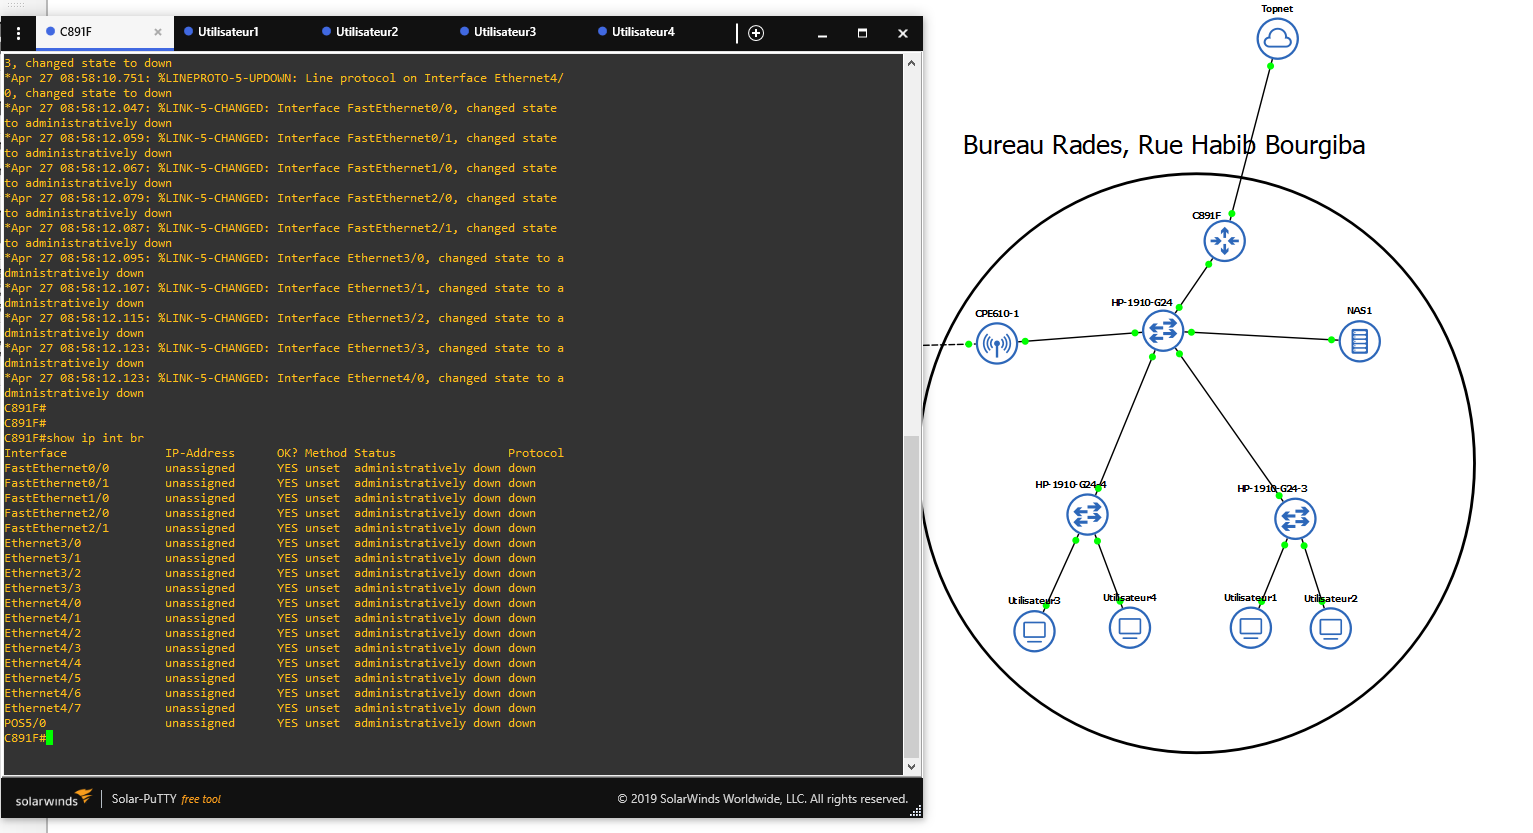
\includegraphics[width=16cm]{Images/BRades-Topologie1.png}
    \caption{Console du routeur de Rades}
    \label{Chap2.2.1}
\end{figure}


Ensuite, dans la figure \ref{Chap2.2.2}, nous avons obtenu une adresse IP DHCP pour notre console et nous avons activé l'option \textit{"domain-lookup"}. 


\begin{figure}[H]
 \centering
    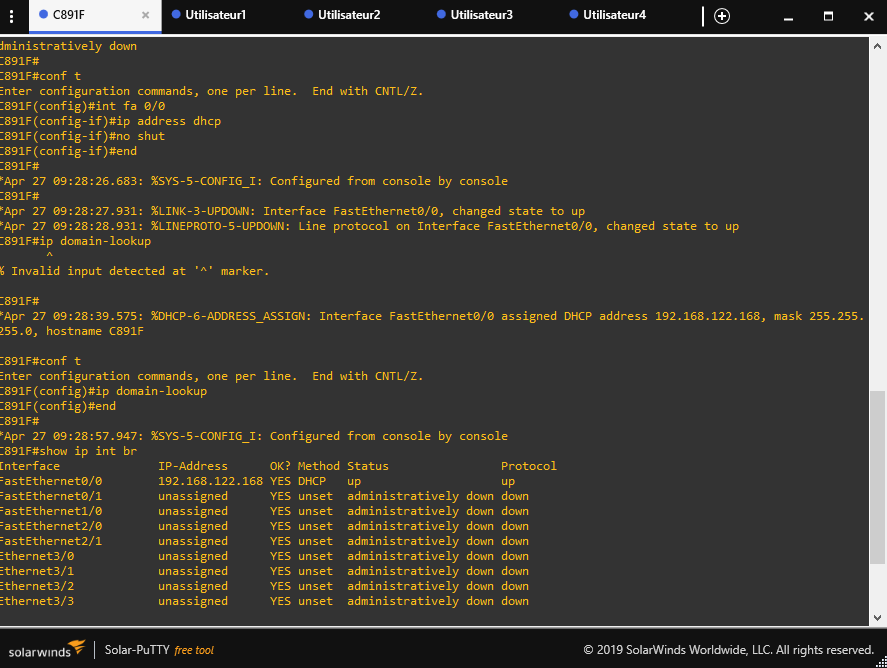
\includegraphics[width=16cm]{Images/BRades-Topologie2.png}
    \caption{Réglage de l'IP adresse}
    \label{Chap2.2.2}
\end{figure}


Dans la figure \ref{Chap2.2.3}, nous effectuons un ping réussi vers "8.8.8.8", ce qui indique que nous avons accès à l'Internet, et également vers "www.google.com" grâce à l'option "domain-lookup" que nous avons utilisée.

\begin{figure}[H]
 \centering
    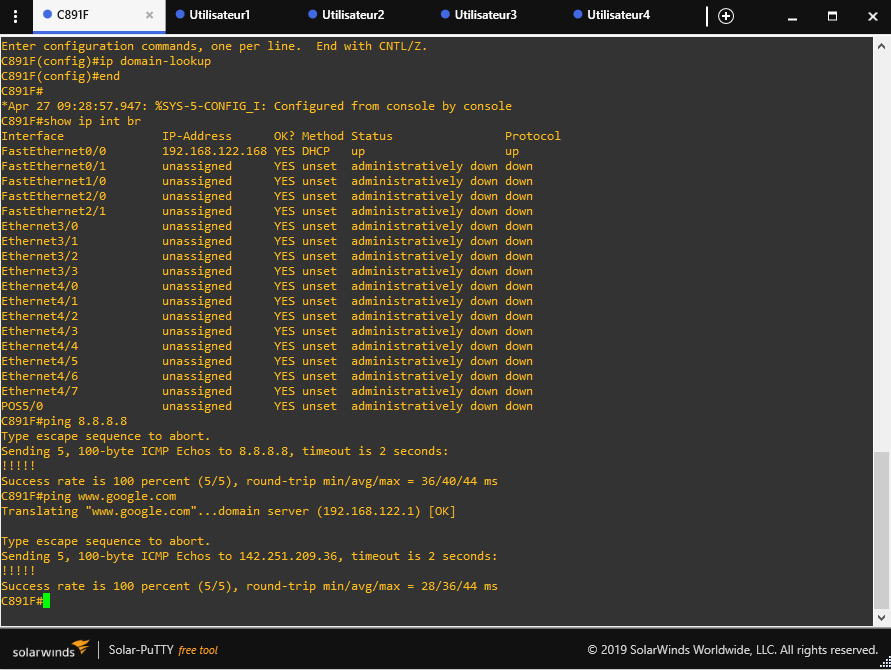
\includegraphics[width=16cm]{Images/BRades-Topologie3.png}
    \caption{Test de connexion de routeur vers l'internet}
    \label{Chap2.2.3}
\end{figure}

Dans la figure \ref{Chap2.2.4}, nous ajoutons un réseau interne (LAN) "192.168.1.1/24" sur le port f0/1. 

\begin{figure}[H]
 \centering
    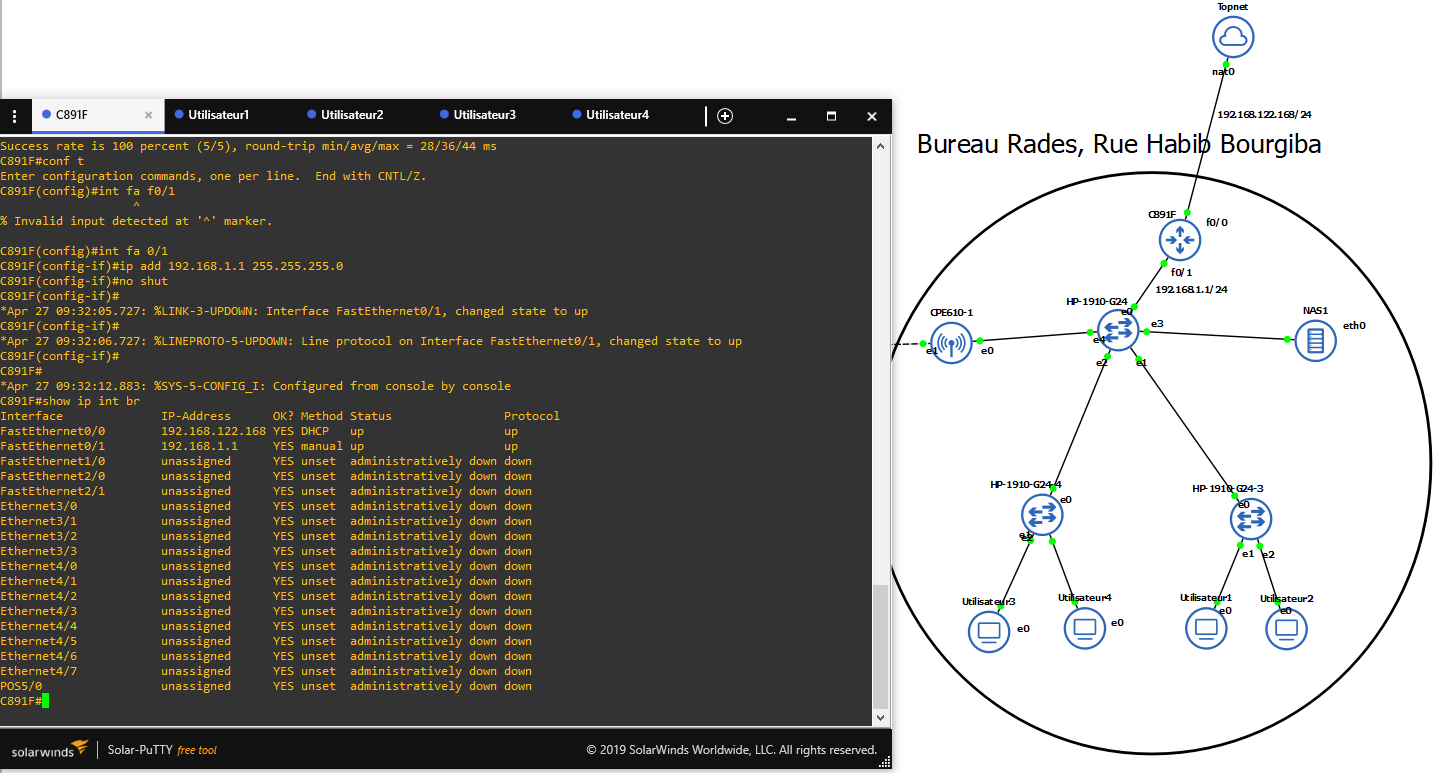
\includegraphics[width=16cm]{Images/BRades-Topologie4.png}
    \caption{Configurer le port f0/1}
    \label{Chap2.2.4}
\end{figure}

Cependant, comme le montre la figure \ref{Chap2.2.5}, nous avons remarqué que l'utilisateur 4 ne pouvait pas toujours accéder à Internet. 

Cela est dû au fait que nous devons configurer notre routeur C891F pour autoriser le trafic du port LAN f0/1 à accéder au WAN port f0/0 (le port de l'internet), et également pour permettre le transfert de tous les protocoles, tels que HTTP et SMTP.




\begin{figure}[H]
 \centering
    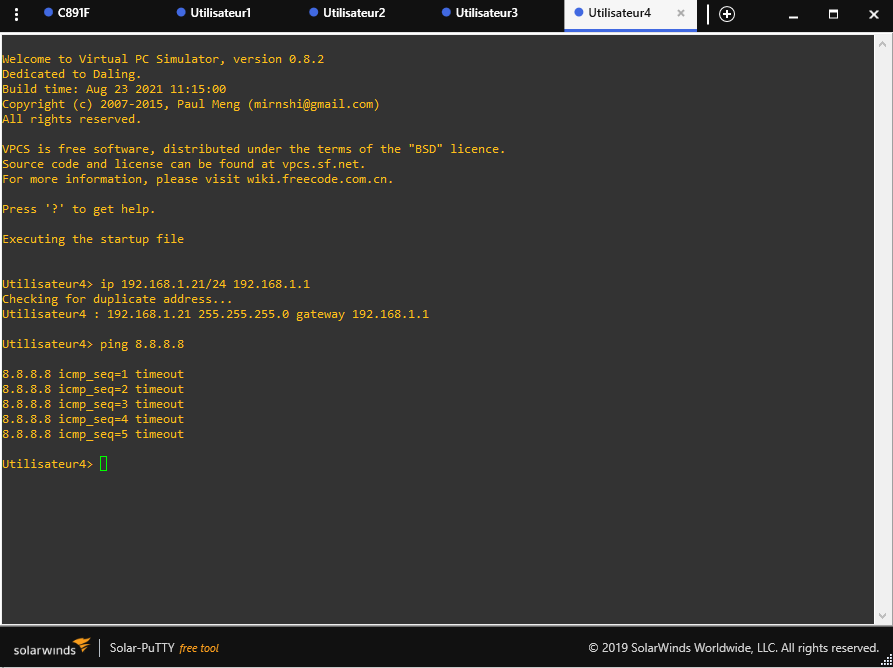
\includegraphics[width=16cm]{Images/BRades-Topologie5.png}
    \caption{Ping de utilisateur4 vers l'internet}
    \label{Chap2.2.5}
\end{figure}


Dans la figure \ref{Chap2.2.6}, nous configurons notre routeur afin d'autoriser la communication entre notre port WAN f0/0 et notre port LAN f0/1.


\begin{figure}[H]
 \centering
    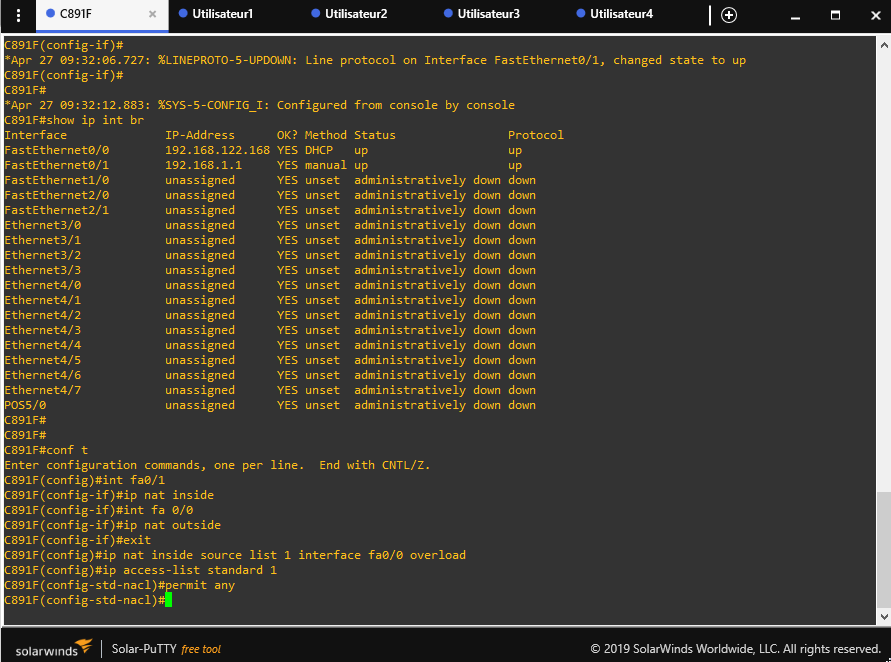
\includegraphics[width=16cm]{Images/BRades-Topologie6.png}
    \caption{Configuration de routeur}
    \label{Chap2.2.6}
\end{figure}


Dans la figure \ref{Chap2.2.7}, nous constatons que toutes les machines avaient accès à internet et pouvaient communiquer entre elles dans le réseau local.

\begin{figure}[H]
 \centering
    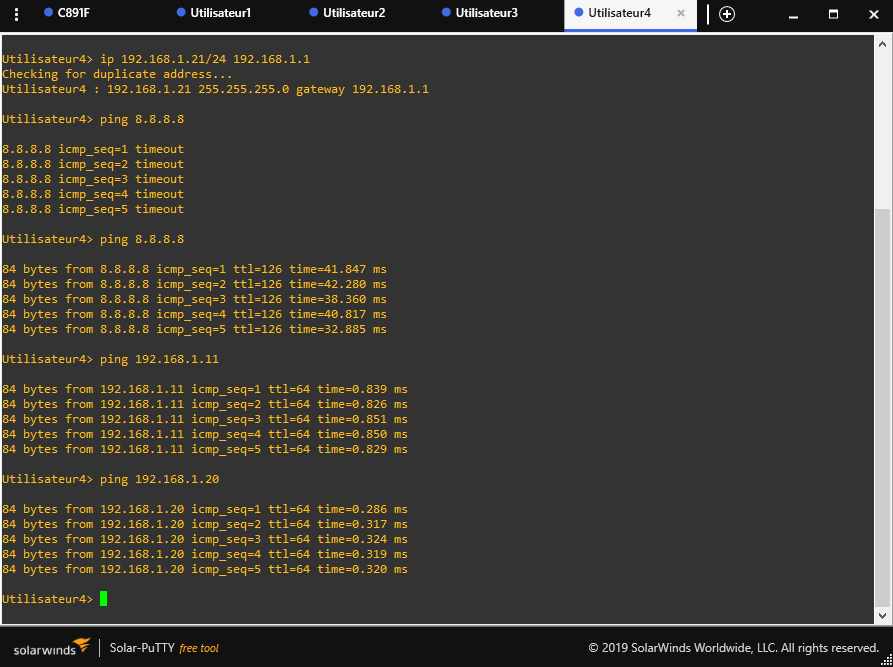
\includegraphics[width=15.5cm]{Images/BRades-Topologie8.png}
    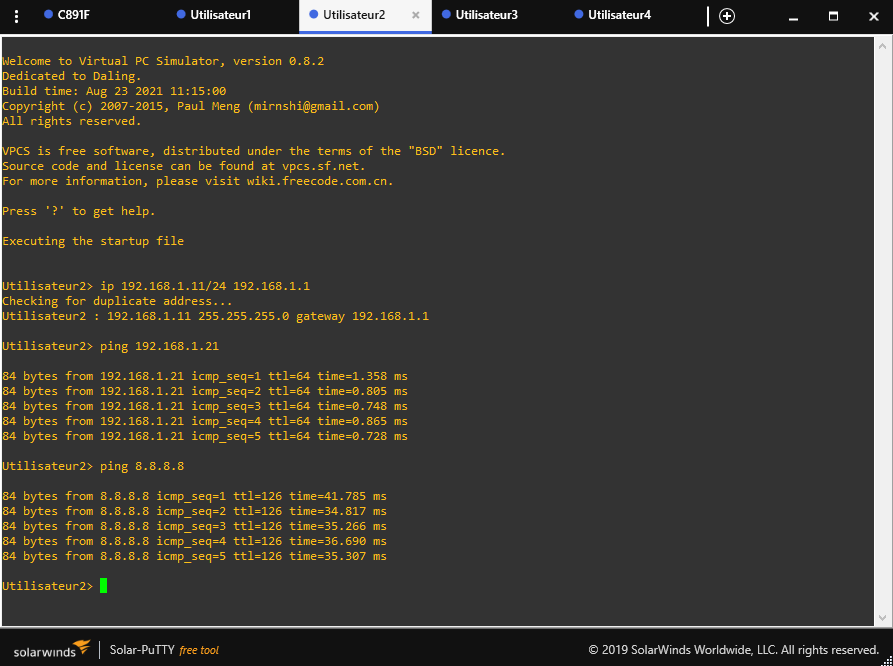
\includegraphics[width=15.5cm]{Images/BRades-Topologie9.png}
    \caption{Test de connexion des utilisateurs}
    \label{Chap2.2.7}
\end{figure}


En résumé, nous avons configuré notre réseau en utilisant GNS3 en étapes, en veillant à ce que toutes les machines aient accès à internet et puissent communiquer entre elles dans le réseau local.


  
\subsection{Implémentation}


Étant donné que l'infrastructure de fibre optique de Topnet/Telecom n'est pas disponible à proximité du bureau central de Rades Melian, nous trouvons une solution en achetant une connexion internet par fibre optique dans deux autres bureaux, Rades (20 Mbps) et Ezzahara (100 Mbps), et en les reliant via un réseau MAN (Metropolitan Area Network). Les deux connexions sont connectées à un routeur Cisco 891F configuré par l'équipe de Topnet, qui distribue le réseau vers un commutateur Cisco v19-10 24G. 


Le routeur Cisco 891F est représenté dans la figure \ref{Chap2.2.10}.

\begin{figure}[H]
\centering
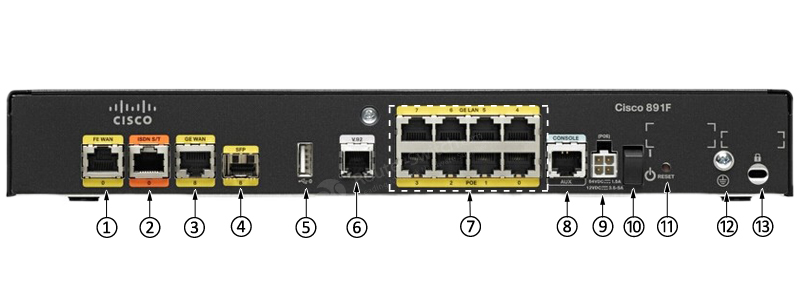
\includegraphics[width=15cm]{Images/C891F_1.jpg}
\caption{Routeur Cisco 891F}
\label{Chap2.2.10}
\end{figure}

À partir du commutateur principale, nous pouvons accéder à d'autres commutateurs qui permettent la connectivité LAN des PC et des objets connectés dans le bureau. La figure \ref{Chap2.2.11} montre l'interconnexion des commutateurs principal et les routeurs pour les bureaux de Rades et Ezzahara.


\begin{figure}[H]
\centering
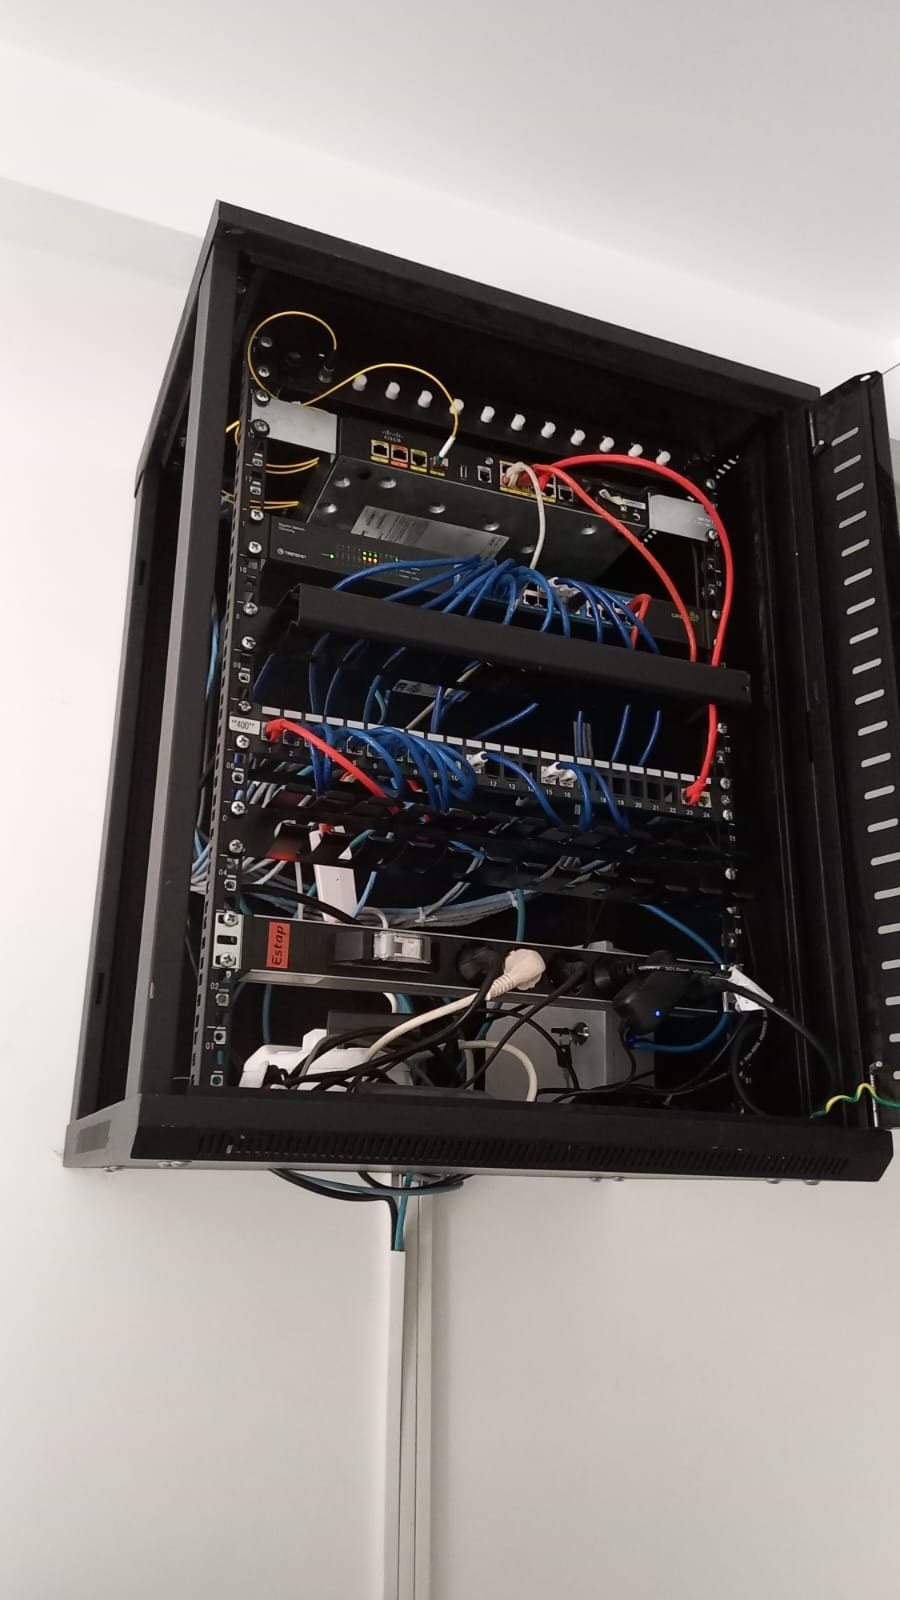
\includegraphics[width=7cm,height=12cm]{Images/BRades-ArmoirePrincipal.jpg} 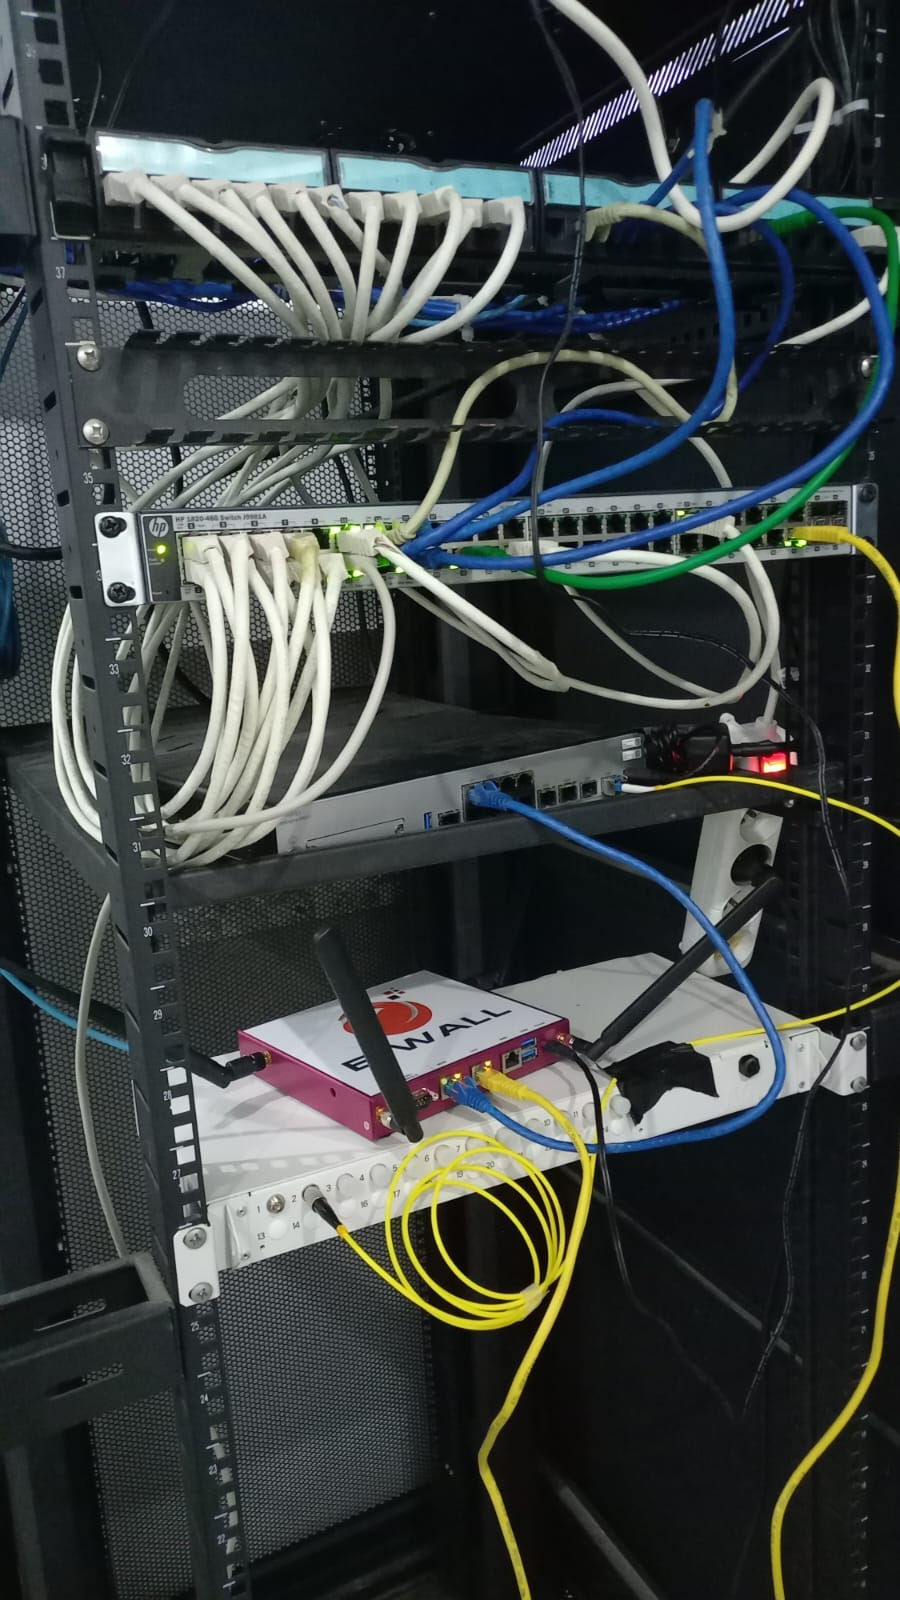
\includegraphics[width=7cm,height=12cm]{Images/Armoire-Ezzahara.jpg} 

\caption{Interconnexion des commutateurs pour les bureaux Rades et Ezzahara}
\label{Chap2.2.11}
\end{figure}



\section{Pare-feu}

Dans cette section, après avoir configuré notre routeur et notre réseau MAN, nous introduisons également un pare-feu dans notre bureau principal à Rades Meliane, ainsi que dans le bureau des développeurs à Ezzahara à l'avenir.


\subsection{Choix pfSense}

Nous choisissons pfSense pour plusieurs raisons essentielles. Tout d'abord, c'est une solution open source, ce qui signifie qu'elle est gratuite et offre une grande flexibilité. De plus, pfSense est reconnu pour sa stabilité et sa fiabilité, en faisant un choix sûr pour sécuriser notre infrastructure. Il bénéficie d'une communauté active et d'une documentation complète, ce qui facilite son utilisation et sa maintenance. En outre, pfSense offre une gamme étendue de fonctionnalités de sécurité, y compris la gestion des règles de pare-feu, la détection d'intrusion, la protection contre les logiciels malveillants, etc. En somme, pfSense est la solution idéale pour renforcer la sécurité de notre réseau tout en offrant souplesse et support actif.


\subsection{Mise en œuvre du pfSense}

Pour déployer pfSense en tant que pare-feu dans notre infrastructure du bureau Rades Melian, qui est la branche principale, nous avons suivi les étapes d'installation suivantes.


Nous utilisons la boîte E-Wall Firewall comme hôte pour notre déploiement de pfSense.


Nous procédons à l'installation de pfSense sur la boîte E-Wall Firewall en suivant les étapes décrites ci-dessous dans les figures de \ref{Chap3.3.2} jusqu'à \ref{Chap3.3.8}.

\begin{figure}[H]
\centering
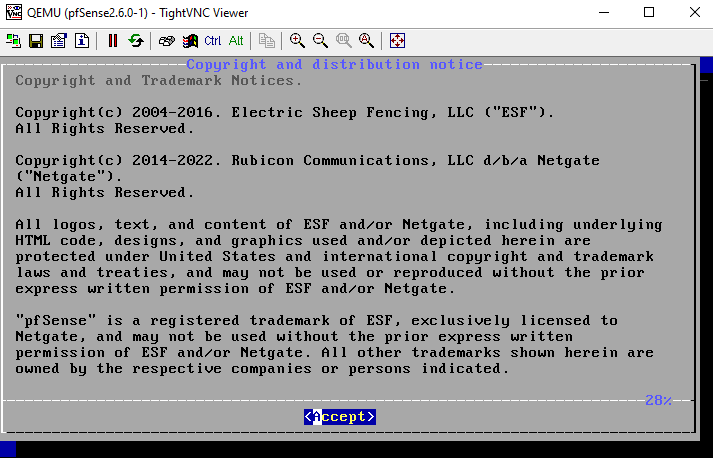
\includegraphics[width=15cm]{Images/BRadesMelian-Topologie2.png}
\caption{Installation de pfSense - Étape 1}
\label{Chap3.3.2}
\end{figure}

\begin{figure}[H]
\centering
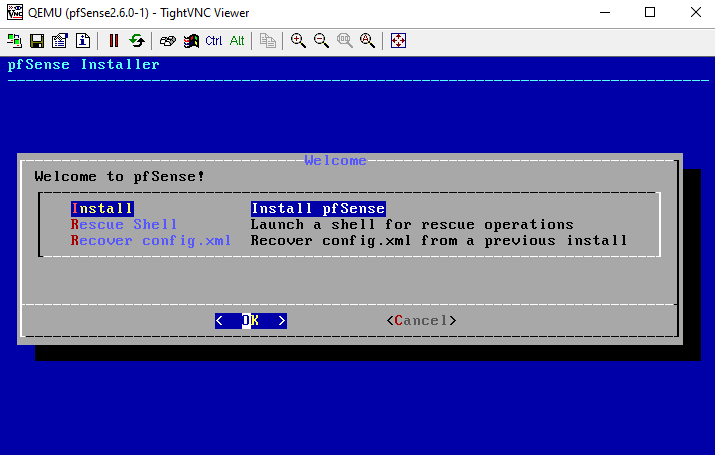
\includegraphics[width=15cm]{Images/BRadesMelian-Topologie3.png}
\caption{Installation de pfSense - Étape 2}
\label{Chap3.3.3}
\end{figure}

\begin{figure}[H]
\centering
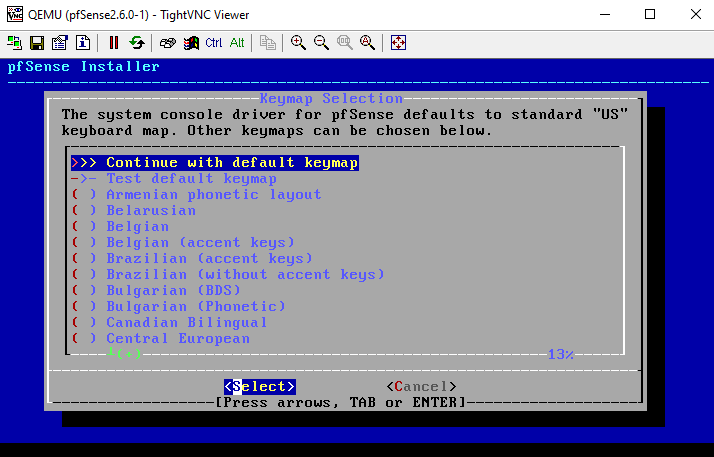
\includegraphics[width=15cm]{Images/BRadesMelian-Topologie4.png}
\caption{Installation de pfSense - Étape 3}
\label{Chap3.3.4}
\end{figure}

\begin{figure}[H]
\centering
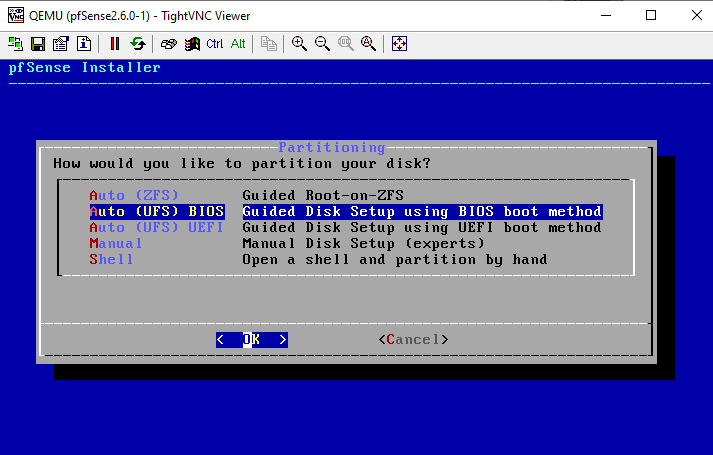
\includegraphics[width=15cm]{Images/BRadesMelian-Topologie5.png}
\caption{Installation de pfSense - Étape 4}
\label{Chap3.3.5}
\end{figure}

\begin{figure}[H]
\centering
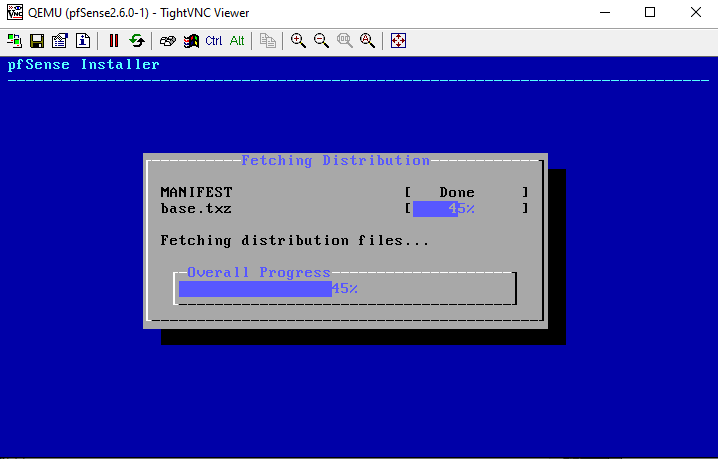
\includegraphics[width=15cm]{Images/BRadesMelian-Topologie6.png}
\caption{Installation de pfSense - Étape 5}
\label{Chap3.3.6}
\end{figure}

\begin{figure}[H]
\centering
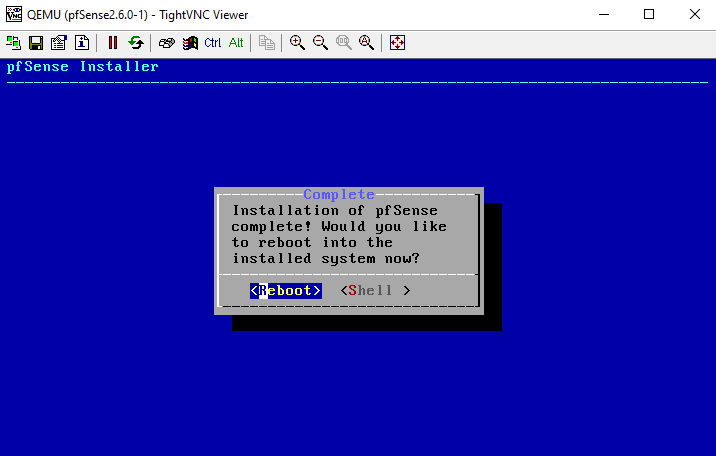
\includegraphics[width=15cm]{Images/BRadesMelian-Topologie7.png}
\caption{Installation de pfSense - Étape 6}
\label{Chap3.3.7}
\end{figure}

\begin{figure}[H]
\centering
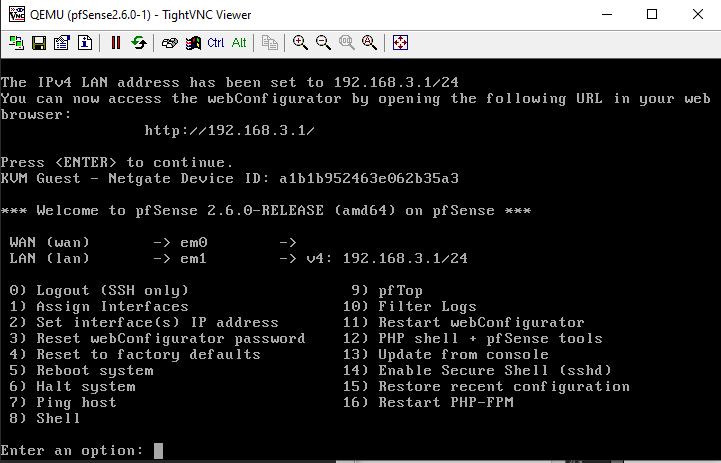
\includegraphics[width=15cm]{Images/BRadesMelian-Topologie8.png}
\caption{Installation de pfSense - Étape 7}
\label{Chap3.3.8}
\end{figure}

\begin{figure}[H]
\centering
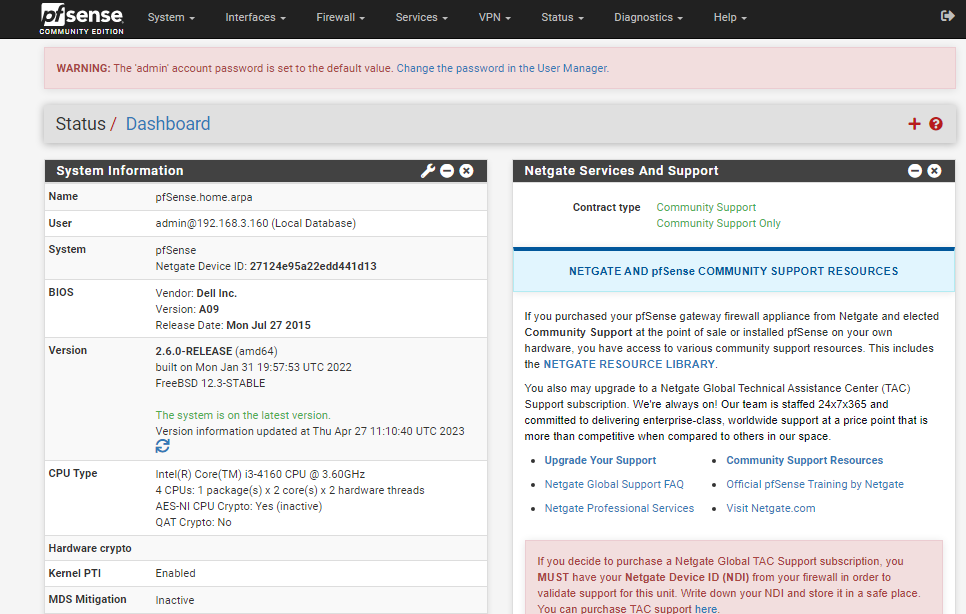
\includegraphics[width=15cm]{Images/BRadesMelian-Topologie14.png}
\caption{Tableau de bord de pfSense}
\label{Chap3.3.9}
\end{figure}

\begin{figure}[H]
\centering
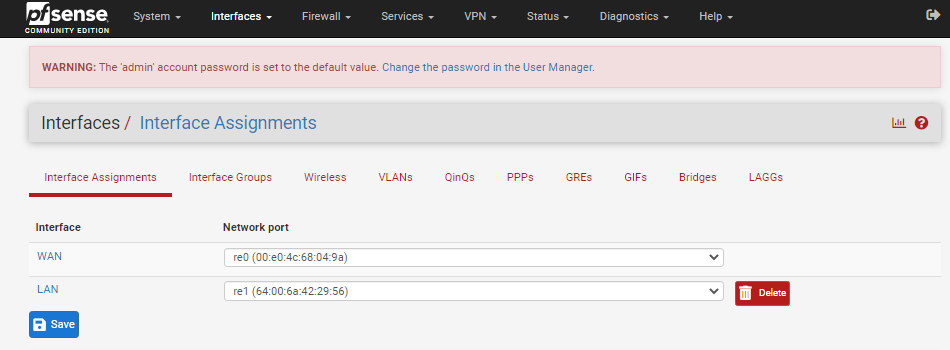
\includegraphics[width=15cm]{Images/BRadesMelian-Topologie15.png}
\caption{Interface de pfSense}
\label{Chap3.3.10}
\end{figure}

Une fois l'installation terminée, nous accédons au tableau de bord de pfSense dans les figures \ref{Chap3.3.9} et \ref{Chap3.3.10} pour configurer les interfaces réseau, les règles de pare-feu et d'autres paramètres de sécurité nécessaires pour protéger notre infrastructure.

pfSense offre une gamme d'options de configuration avancée, notamment la gestion des interfaces, les règles de pare-feu, les services VPN, la surveillance du trafic, etc. 

En utilisant ces fonctionnalités, nous pouvons personnaliser notre pare-feu pour répondre à nos exigences spécifiques de sécurité et de réseau.

\section{Conclusion}

En résumé, la création de l'infrastructure informatique pour notre projet a exigé une analyse approfondie des besoins de l'entreprise ainsi qu'une sélection méticuleuse des outils et des technologies pour établir une infrastructure à la fois robuste et sécurisée. 

Nous avons soigneusement examiné les différentes architectures réseau, englobant le réseau local, le réseau MAN, et les configurations spécifiques pour les trois bureaux.

Ce chapitre nous a permis de détailler les diverses étapes du déploiement de l'infrastructure IT pour le projet. Dans le prochain chapitre, nous aborderons le déploiement du système d'information pour compléter notre approche globale visant à répondre aux besoins de l'entreprise, tout en garantissant la sécurité et la solidité de notre infrastructure.








